% Create a Table of Contents in Beamer
\documentclass[10pt,t]{beamer}
% Theme choice:
\usetheme{Singapore}
\useoutertheme{sidebar}
\usecolortheme{seahorse}
\setbeamercolor{titlelike}{bg=white}
\setbeamercolor{frametitle}{bg=white}
%\setbeamertemplate{frametitle}[default][left]
\setbeamertemplate{navigation symbols}{}
\setbeamertemplate{footline}{\begin{flushright}\small \insertframenumber\end{flushright}}

\usepackage{graphicx}
\usepackage{amsmath}
\usepackage{amsfonts}
\usepackage{amssymb}
\usepackage{amsthm}
\usepackage[normalem]{ulem}
\usepackage{hyperref}

\newcommand\tab[1][1cm]{\hspace*{#1}}

% Title page details: 
\title{Chapter 4: Regression for binary outcomes} 
\author{Nina Galanter}
\date{\today}



\begin{document}
	% Title page frame
	\begin{frame}
	\titlepage 
\end{frame}

\begin{frame}{Learning objectives}
	By the end of Chapter 2, you should be able to: 
	\begin{itemize}
		\item Distinguish between probability and odds and know how to calculate each in \texttt{R}
		\item Describe the measures of association used for binary outcomes and exposures of interest
		\item Formulate a regression model, given a scientific or statistical question about a binary outcome
		\item Interpret the coefficients (along with confidence intervals and p-values) of a regression model for a binary outcome
		\item Describe how (and why) logistic regression interpretation changes when we have data from a case-control study
		\item Use \texttt{R} to fit a logistic regression model and produce supporting figures/tables
	\end{itemize}
\end{frame}

%Outline frame
\begin{frame}{Outline}
\tableofcontents
\end{frame}

\AtBeginSection[ ]
{
\begin{frame}{Outline}
\tableofcontents[currentsection]
\end{frame}
}

\AtBeginSubsection[ ]
{
	\begin{frame}{Outline}
		\tableofcontents[currentsubsection]
	\end{frame}
}


% Presentation structure
\section{Binary outcomes}

% quantitative outcomes from ch1
\begin{frame}{Recall: Variable type}
	In Chapter 1, we asked scientific questions involving quantitative outcomes: those that have a fundamentally numeric quality: 
	\\~\
	
	\begin{itemize}
		\item Our primary outcomes of interest were \textcolor{blue}{birthweight} and \textcolor{blue}{atrophy score}
		\bigskip
		
		\item We also saw examples involving FEV, 100m dash times, dental patient pain ratings
	\end{itemize}
\end{frame}

% binary variable examples
\begin{frame}{Recall: Variable type}
Binary variables are a type of \textcolor{blue}{categorical} variable with two possible categories. We often implicitly think of them in a 0-1 sense, but they often don't have actual numeric value. 
\\~\

Examples we often see in biomedical research: 
\medskip

\begin{itemize}
	\item Type I diabetes (presence/absence)
	\medskip
	
	\item Surgery complications (occurred/did not occur)
	\medskip
	
	\item Smoking (yes/no)
	\medskip
	
	\item Mortality prior to age 5 (occurred/did not occur)
	\medskip
	
	\item COVID status (positive/negative)
\end{itemize}
\end{frame}

% binary variable scientific questions
\begin{frame}{Scientific questions about binary variables}
	Questions we could ask about these variables include
	\medskip
	
	\begin{itemize}
		\item Are variants in the HLA-DRB1 gene associated with \textcolor{blue}{Type I diabetes}? 
		\medskip
		
		\item Are \textcolor{blue}{surgery complications} after upper endoscopy associated with who (anesthesiologist vs nurse) performed the sedation?
		\medskip
		
		\item Is the use of e-cigarettes associated with \textcolor{blue}{smoking}?
		\medskip
		
		\item Is having an HIV positive birth parent associated with the risk of \textcolor{blue}{neonatal mortality}?
		\medskip
		
		\item Is Vitamin D intake associated with the risk of \textcolor{blue}{testing positive for COVID}?
		\medskip
		
	\end{itemize}
\end{frame}

\begin{frame}{Scientific questions about binary variables}
	One specific question that we will study is:

		\bigskip
		
\textcolor{blue}{Are monetary incentives associated with choosing to receive HIV test results?}

	\vspace{0.7cm}
	
	\begin{itemize}
		\item HIV continues to be a serious health challenge worldwide
		\medskip
		
		\item People knowing their HIV status is important in both successfully treating the disease and preventing transmission
		
		\medskip
		
		\item However, there can be psychological, social\footnote{Thornton, Rebecca L. 2008. 'The Demand for, and Impact of, Learning Hiv Status.' American Economic Review 98 (5): 1829–63}, and logistical barriers to learning one's HIV status
	\end{itemize}
\end{frame}

\begin{frame}{The Thornton HIV Study}
	\vspace{-10 mm}
	
	This study was part of a larger collaborative project between the University of Pennsylvania and the Malawi College of Medicine.
	
	\medskip
	
	The project is taking place in Malawi. In 2020, researchers estimated that HIV prevalence among adults in Malawi is 8.9\%, or about 946,000 adults. They also estimated that 88.3\% of those adults living with HIV know their HIV status, which is below the UNAIDS 2025 target of 95\%\footnote{https://phia.icap.columbia.edu/second-population-survey-assessing-hiv-in-malawi-shows-progress-toward-epidemic-control/}.
	
	\medskip
	
	In this particular study\footnote{Thornton, Rebecca L. 2008. 'The Demand for, and Impact of, Learning Hiv Status.' American Economic Review 98 (5): 1829–63}, conducted in 2004, nurses knocked on doors throughout Malawi offering free in-home testing for HIV. Participants then were given randomly selected vouchers for between 0-3 USD to redeem if they went to a test result center to retrieve their result.
	
	\smallskip
	
	\textcolor{violet}{\textbf{Pollev:}} What study design is this?
	\tiny{\url{https://PollEv.com/multiple_choice_polls/yNK1Wz10JvX1bKaV67QPe/respond}}
	\normalsize
	
	\textcolor{blue}{\textbf{Answer:}} Experiment
\end{frame}

\begin{frame}{Recall: summarizing a binary variable}
	Let's think about receiving an incentive and choosing to get a HIV result. 
	\\ ~\ 
	
	We can talk about the \textcolor{blue}{probability} of getting a result among those who received an incentive ($p_A$) and the probability of getting a result among those do did not receive an incentive ($p_B$).
	\medskip
	
	\begin{itemize}
		\item Generally, ``probability," ``risk," ``proportion" refer to the same quantity.
		
		\medskip
	\end{itemize}  

	\textcolor{blue}{Odds} are defined as $\frac{p}{1-p}$, where $p$ is a probability.
	\medskip
	
	\begin{itemize}
		\item Odds of getting a result with an incentive: $\frac{p_A}{1-p_A}$
		
		\medskip
		
		\item Odds of getting a result without an incentive: $\frac{p_B}{1-p_B}$
	\end{itemize}
\end{frame}

\begin{frame}{Recall: summarizing a binary variable}
\textcolor{blue}{Probability}:
\medskip

\begin{itemize}
	\item Takes values in $[0,1]$.
	\medskip
	
	\item Generally more intuitive than odds. 
	\medskip
	
	\item In some study designs, impossible to estimate! (More on this later.)
\end{itemize}   
\medskip

\textcolor{blue}{Odds}:
\medskip
\begin{itemize}
	\item Take values in $(0,\infty)$.
	\medskip
	
	\item Are less intuitive for most people (unless you do a lot of betting).
	\medskip
	
	\item Can be estimated from most common biomedical study designs. 
\end{itemize}
\end{frame}

\begin{frame}{Odds and Probability in HIV Data}
	\vspace{-5 mm}
	
	\begin{table}
		\centering
	\begin{tabular}{cc|c|c|}
		&Results &No & Yes\\
		Incentive& && \\
		\hline
		No &&410&211\\\hline
		Yes &&461&1743
	\end{tabular}
\end{table}
\smallskip

\textcolor{blue}{Probability of results among those who received incentive:}\\ $\frac{1743}{1743+461}\approx$ 79\%
\bigskip

\textcolor{blue}{Probability of results among those who did not receive incentive:}\\ $\frac{211}{211+410}\approx$ 34\%
\bigskip

\textcolor{blue}{Odds of results among those who received incentive:}\\ $\frac{1743}{461}\approx$ 3.78
\bigskip

\textcolor{blue}{Odds of results among those who did not receive incentive:}\\ $\frac{211}{410}\approx$ 0.51

\end{frame}

\begin{frame}{Measures of association}
	We can now describe the \textcolor{blue}{probability} or \textcolor{blue}{odds} of choosing to get results among those who did and did not receive an incentive. 
	\\ ~\
	
	\textbf{Scientific question:} Is receiving an incentive \textcolor{blue}{associated} with choosing to get a result? 
	\\ ~\
	
	In order to do statistics, we need to clarify what \textcolor{blue}{associated} means for binary variables.
\end{frame}

\begin{frame}{Measures of association}
\textcolor{blue}{Equal probabilities}: If $p_A = p_B$, then
\medskip

	\begin{itemize}
		\item \textcolor{blue}{Risk difference}: $p_A - p_B = 0$
		\medskip
		
		\item \textcolor{blue}{Relative risk}: $\frac{p_A}{p_B} = 1$
	\end{itemize}  
\bigskip

\textbf{Risk difference is an absolute measure, while relative risk is a relative measure.}

\bigskip

\textcolor{blue}{Equal odds}: If $\frac{p_A}{1-p_A} = \frac{p_B}{1-p_B}$, then
\medskip 
	\begin{itemize}
		\item \textcolor{blue}{Odds ratio}: $\frac{\frac{p_A}{1-p_A}}{\frac{p_B}{1-p_B}}=1$ 
	\end{itemize}
\bigskip

These are the most common measures of association for binary outcomes. 
\end{frame}

\begin{frame}{Relative risk versus Odds ratio}
	\begin{itemize}
		\item Relative risk and odds ratio will always be in the \textcolor{blue}{same direction} (either above or below 1)
		\medskip
		\item Odds ratio will always be \textcolor{blue}{more extreme} than relative risk (in terms of distance from 1)
	\end{itemize}
\end{frame}

\begin{frame}{Measures of association}
When we are approaching a scientific question about association, we need to think about
\medskip

\begin{itemize}
	\item \textcolor{blue}{Summary measure:} Probability or odds
	\medskip
	\item \textcolor{red}{Contrast:} Difference or ratio
\end{itemize}
\vspace{0.5cm}  
In our running example:
\medskip
\begin{itemize}
	\item Is there a \textcolor{red}{difference} in the \textcolor{blue}{probability} of choosing to get a result between people who receive an incentive and those who do not?  
	\medskip
	
	\item Is the \textcolor{red}{ratio} of \textcolor{blue}{probabilities} of choosing to get a result, comparing people who do and do not receive an incentive, equal to 1?  
	\medskip
	
	\item Is the \textcolor{red}{ratio} of \textcolor{blue}{odds} of choosing to get a result, comparing people who do and do not receive an incentive, equal to 1? 
\end{itemize}
\end{frame}

\begin{frame}{Measure of Association for HIV Data}
	
		\vspace{-8 mm}
	
	\begin{table}
		\centering
		\begin{tabular}{cc|c|c|}
			&Results &No & Yes\\
			Incentive& && \\
			\hline
			No &&410&211\\\hline
			Yes &&461&1743
		\end{tabular}
	\end{table}
	\smallskip
	
	\textcolor{blue}{Risk difference of getting results between those who did and did not receive an incentive:}
	
	\medskip
	\large
	 $\frac{1743}{1743+461}-\frac{211}{211+410}\approx$ 45\%
	\medskip
	\normalsize
	
	\textcolor{blue}{Relative risk of getting results comparing those who did and did not receive an incentive:}
	
	\large
	\medskip
	 $\frac{\frac{1743}{1743+461}}{\frac{211}{211+410}}\approx$ 2.33
	\medskip
	\normalsize
	
	\textcolor{blue}{Odds ratio of getting results comparing those who did and did not receive an incentive:}
	
	\large
	\medskip
	 $\frac{\frac{1743}{461}}{\frac{211}{410}}\approx$ 7.35

	
\end{frame}



% Linear regression
\section{Linear regression with binary outcomes}


\begin{frame}
	\frametitle{Simple linear regression with a binary outcome}
	Can we use linear regression to look at the association between an exposure and a binary outcome? Yes!
	\medskip
	
	\textbf{\textcolor{orange}{Though this is rarely done in practice.}}
	
	\bigskip
	

	
	A simple linear regression model: $E[Y \mid X] = \beta_0 + \beta_1 X$.
\medskip

		\begin{itemize}
			\item Recall: $E[Y \mid X]$ is the \textcolor{blue}{\textit{expected value}} (average) of $Y$ given $X$ 
		\end{itemize}

	 \bigskip
	 
	What's the average of a binary variable $Y$?   
	
	\medskip
	\textit{It's the probability that $Y$ equals 1!} $\left(\text{i.e., } E[Y] = \text{P}(Y=1)\right)$  
	\bigskip
	
	The sample probability and sample means are also equal:
	
\[\hat{p} = \hat{\text{P}}(Y=1) = \frac{y_1+y_2+...+y_n}{n} = \overline{Y} \]

\end{frame}

\begin{frame}
	\frametitle{Simple linear regression with binary outcomes}
	
		\vspace{-5 mm}
	
	In the HIV study example, \textcolor{blue}{\texttt{results}} is a binary variable which indicates whether subjects chose to get their test results (\textcolor{blue}{the outcome}), and \textcolor{violet}{\texttt{incentive}} is the binary variable which indicates whether subjects received any incentive (\textcolor{violet}{the exposure}).
	
	\medskip
	
	\textbf{Discuss with your neighbor:} 
\medskip

	
	% recall activity
	Suppose we fit the simple linear regression model $$E[\texttt{results} \mid \texttt{incentive}] = \beta_0 + \beta_1 \texttt{incentive}$$ 
	
	What is the interpretation for the coefficients in this model?
	\medskip
	
	\begin{enumerate}
			\item $\beta_0$
			\medskip
			\item $\beta_1$
		\end{enumerate} 
\end{frame}

\begin{frame}
	\frametitle{Simple linear regression with binary outcomes}
	
	\vspace{-5 mm}
	
	In the HIV study example, \textcolor{blue}{\texttt{results}} is a binary variable which indicates whether subjects chose to get their test results (\textcolor{blue}{the outcome}), and \textcolor{violet}{\texttt{incentive}} is the binary variable which indicates whether subjects received any incentive (\textcolor{violet}{the exposure}).
	
	\medskip
	
	\textbf{Discuss with your neighbor:} 
	\medskip
	
	
	% recall activity
	Suppose we fit the simple linear regression model $$E[\texttt{results} \mid \texttt{incentive}] = \beta_0 + \beta_1 \texttt{incentive}$$ 
	
	What is the interpretation for the coefficients in this model?
	\medskip
	
	\begin{enumerate}
		\item $\beta_0$ : {The probability of getting a result among those who do not receive an incentive}
		\medskip
		\item $\beta_1$ : {The \textcolor{blue}{risk difference} of getting a result comparing those who do and do not receive an incentive}
	\end{enumerate} 

\medskip
	\textbf{Linear regression allows us to look at association via the \textcolor{blue}{risk difference}}

\end{frame}


\begin{frame}{Potential issues}
	
	\begin{itemize}
	\item Predictions for linear regression can fall outside of [0,1]
	
	\medskip
	
	\item For traditional linear regression, we assume equal variance across predictor values, but a binary variable with mean (probability) of $p$ has variance $p(1-p)$. 
	\medskip
	\begin{itemize}
	\item  If we're claiming that $E[Y \mid X] = \beta_0 + \beta_1X$, we're also implying that $\text{Var}[Y \mid X] = (\beta_0 + \beta_1 X)(1 - \beta_0 - \beta_1 X)$. 
	\medskip
	
	\item But linear regression assumes that $\text{Var}[Y \mid X] = \sigma^2$, which doesn't depend on $X$!
	
	\medskip
	
	\item \textit{We could use robust standard errors to deal with this.}
	

	\end{itemize}
\end{itemize}
\medskip

\textcolor{blue}{Because of these issues, linear regression is rarely used for binary outcomes in practice.}

\medskip

\textcolor{blue}{\textbf{So what can we do instead?}}

\end{frame}


%
%
%%%% LOGISTIC REGRESSION %%%
\section{Logistic regression}

\subsection{Simple logistic regression}




% motivating logistic regression
\begin{frame}
	\frametitle{HIV data: odds}
	\vspace{-0.5cm}
	\begin{small} What if we wanted to quantify the association between receiving an incentive and choosing to get HIV test results via the \textcolor{blue}{odds ratio} rather than the risk difference? \end{small}   \vspace{0.1cm}

	\begin{enumerate}
			\item \textbf{Scientific Question:} Are cash incentives \textcolor{orange}{associated} with the probability of choosing to get HIV results?  
			\item \textbf{Statistical Question:} is the \textcolor{orange}{ratio of odds} of getting test results between people who do and do not receive cash incentives different from 1?  
			\begin{itemize}
					\item \textbf{Parameter:} odds ratio  
				\end{itemize}
			\item Take a \textbf{sample} from the population: randomized trial of people in Malawi in 2004 
			\item Perform \textit{statistical inference}:
			\begin{itemize}
					\item Calculate a corresponding \textbf{statistic}: \textcolor{blue}{sample odds ratio}
					\item Quantify uncertainty in your statistic
					\item Perform a hypothesis test  
				\end{itemize}
		\end{enumerate}
	
	\vspace{0.1cm}
	We can use \textcolor{blue}{logistic} regression to answer this question!
\end{frame}

\begin{frame}{Thinking on the odds scale}
	As we've seen, the odds can take values from 0 to $\infty$. 
	\\ ~\
	
	Fitting a regression model on a variable with a restricted range can cause issues with values falling outside the possible range. We saw this a few slides ago with linear regression!
	\\ ~\
	
	Solution: Apply the $log$ function to the odds. 
	%%% INSERT FIGURE HERE
\end{frame}

\begin{frame}{Brief review of logarithms}
	\vspace{-0.6cm}
	In statistics, we generally deal with the natural logarithm, which has base $e$. You may have seen this written as \textcolor{blue}{$\ln$}, but we will use \textcolor{blue}{$\log$}. 
	\\ ~\
	
	The logarithm of $x$ is the number $b$ such that $e^b = x$, i.e. the power to which you raise $e$ to get $x$. 
	\\ ~\
	
	This might seem like an odd function to use, but logarithms take nonnegative numbers and map them to $(-\infty, \infty)$, which lets us not worry about restricted ranges. 
	
	\begin{center}
		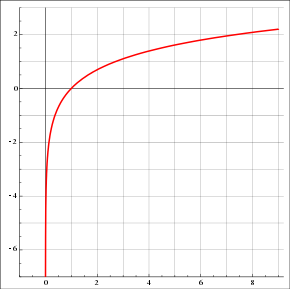
\includegraphics[width=0.4\textwidth]{./figs/log}
	\end{center}
\end{frame}

\begin{frame}{Brief review of logarithms}
	Two very useful properties of logarithms we will use: 
	
	\medskip
	
	\begin{itemize}
		\item The logarithm is the inverse of the exponential function:
		\begin{align*}
			e^{\log(x)} = x \tab \text{and} \tab \log(e^x) = x
		\end{align*}
	\medskip
		\item The logarithm of a quotient is the difference of the logarithms:
		\begin{align*}
			\log(x/y) = \log(x) - \log(y)
		\end{align*}
	\end{itemize}
\end{frame}

% simple logistic regression recall
\begin{frame}{Simple logistic regression: interpretation}
	\textbf{Discuss with your neighbor:}
	\\ ~\
	
	Suppose we fit the simple logistic regression model $$\log\left(\text{Odds}[\texttt{results} \mid \texttt{incentive}]\right) = \beta_0 + \beta_1 \texttt{incentive},$$ What is the interpretation of the following quantities?
	\medskip
	\begin{enumerate}
		\item $\beta_0$
		\medskip
		\item $\beta_1$
		\medskip
		\item $\exp(\beta_0)$
		\medskip
		\item $\exp(\beta_1)$
	\end{enumerate} 
\end{frame}

% simple logistic regression recall
\begin{frame}{Simple logistic regression: interpretation}
	Suppose we fit the simple logistic regression model $$\log\left(\text{Odds}[\texttt{results} \mid \texttt{incentive}]\right) = \beta_0 + \beta_1 \texttt{incentive},$$ What is the interpretation of the following quantities?
	\medskip
	\begin{enumerate}
		\item \textcolor{blue}{$\beta_0$}: log odds of $\texttt{results} = 1$ when $\texttt{incentive} = 0$
		$$\log\left(\text{Odds}[\texttt{results}  =1 \mid \texttt{incentive} = 0]\right) = \beta_0 + \beta_1\times 0$$\\
		
		\textcolor{blue}{$\beta_0$ is the log odds of getting a result among people who do not receive an incentive.}
	\end{enumerate} 
\end{frame}

% simple logistic regression recall
\begin{frame}{Simple logistic regression: interpretation}
	Suppose we fit the simple logistic regression model $$\log\left(\text{Odds}[\texttt{results} \mid \texttt{incentive}]\right) = \beta_0 + \beta_1 \texttt{incentive},$$ What is the interpretation of the following quantities?
	
	\medskip
	
	\begin{enumerate}
		\item[2.] \textcolor{blue}{$\beta_1$}: difference in log odds of $\texttt{results} = 1$ comparing $\texttt{incentive} = 1$ and $\texttt{incentive} =0$ groups
	\end{enumerate} 

	\begin{align*}
	&\log\left(\text{Odds}[\texttt{results} =1 \mid \texttt{incentive} = x+1]\right) = \beta_0 + \beta_1(x+1)\\
	&-\log\left(\text{Odds}[\texttt{results} =1 \mid \texttt{incentive} = x + 1]\right) = \beta_0 + \beta_1x \\
	&= \beta_1
\end{align*}

\medskip

\textcolor{blue}{$\beta_1$ is the log odds ratio of getting HIV test results comparing those with and without an incentive}

\end{frame}

% simple logistic regression recall
\begin{frame}{Simple logistic regression: interpretation}
	Suppose we fit the simple logistic regression model $$\log\left(\text{Odds}[\texttt{results} \mid \texttt{incentive}]\right) = \beta_0 + \beta_1 \texttt{incentive},$$ What is the interpretation of the following quantities?
	\medskip
	\begin{enumerate}
		\item[3.] \textcolor{blue}{$\exp(\beta_0)$}: odds of $\texttt{results} = 1$ when $\texttt{incentive} = 0$
		$$\text{Odds}[\texttt{results}  =1 \mid \texttt{incentive} = 0] = \exp(\beta_0 + \beta_1\times 0)$$\\
		
		\textcolor{blue}{$\exp(\beta_0)$ is the odds of getting a result among people who do not receive an incentive.}
	\end{enumerate} 
\end{frame}

% simple logistic regression recall
\begin{frame}{Simple logistic regression: interpretation}
	
	\vspace{-5 mm}
	
	Suppose we fit the simple logistic regression model $$\log\left(\text{Odds}[\texttt{results} \mid \texttt{incentive}]\right) = \beta_0 + \beta_1 \texttt{incentive},$$ What is the interpretation of the following quantities?
	\medskip
	\begin{enumerate}
		\item[4.] \textcolor{blue}{$\exp(\beta_1)$}: ratio of odds of $\texttt{results} = 1$ comparing $\texttt{incentive} = 1$ and $\texttt{incentive} = 0$ groups
	\end{enumerate} 
\begin{footnotesize}
	\begin{align*}
		&\log\left(\text{Odds}[Y =1 \mid X = x + 1]\right) - \log\left(\text{Odds}[Y =1 \mid X = x ]\right) = \beta_1\\
		&\Rightarrow \exp(\log\left(\text{Odds}[Y =1 \mid X = x + 1]\right) - \log\left(\text{Odds}[Y =1 \mid X = x ]\right)) = \exp(\beta_1)\\
		&\Rightarrow \exp\biggr(\log\biggr(\frac{\text{Odds}[Y =1 \mid X = x + 1]}{\text{Odds}[Y =1 \mid X = x ]}\biggr)\biggr) = \exp(\beta_1)\\
		&\Rightarrow \frac{\text{Odds}[Y =1 \mid X = x + 1]}{\text{Odds}[Y =1 \mid X = x ]} = \exp(\beta_1)
	\end{align*}
	\medskip
	\normalsize
	
	\textcolor{blue}{$\exp(\beta_1)$ is the odds ratio of getting HIV test results comparing those with and without an incentive}
	
\end{footnotesize}
\end{frame}

% simple logistic regression recall
\begin{frame}{Simple logistic regression: interpretation}
	Suppose we fit the simple logistic regression model $$\log\left(\text{Odds}[Y =1 \mid X]\right) = \beta_0 + \beta_1 X,$$ where our outcome $Y$ is binary. What is the interpretation of the following quantities?
	\medskip
	
	\begin{enumerate}
		\item $\beta_0$: log odds of $Y = 1$ when $X = 0$  
		\item $\beta_1$: difference in log odds of $Y = 1$ comparing $X = 1$ and $X =0$ groups  
		\item $\exp(\beta_0)$: odds of $Y = 1$ when $X = 0$  
		\item $\exp(\beta_1)$: ratio of odds of $Y = 1$ comparing $X = 1$ and $X = 0$ groups (\textcolor{blue}{in other words, the odds ratio!})
	\end{enumerate} 
\end{frame}

\begin{frame}{Another motivation for logistic regression}
	
	\vspace{-5 mm}
	
	\textcolor{red}{Issue}: Linear prediction for binary outcomes can lead to predictions outside of (0,1), as the range of a line is all real numbers.
	
	\medskip
	
	\textcolor{blue}{Solution}: The logistic function takes any real number and maps it to (0,1). 
	
	\begin{figure}
		\centering
		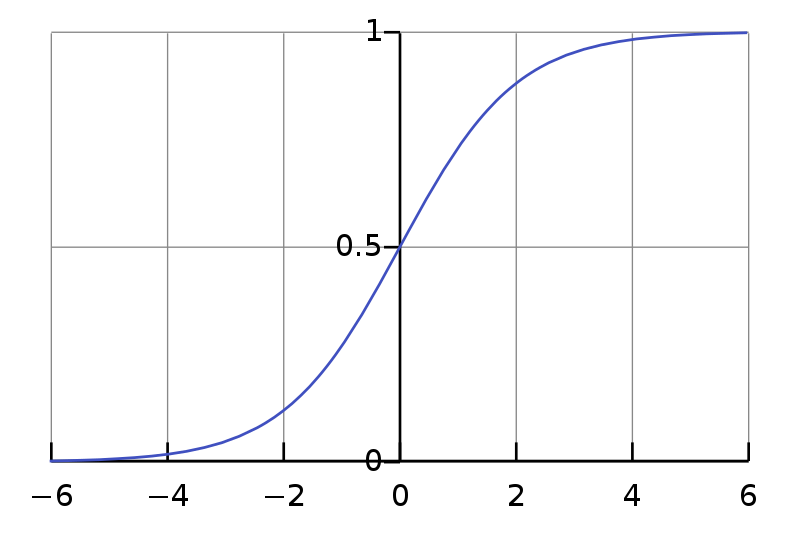
\includegraphics[scale = 0.15]{figs/logistic_curve}
	\end{figure}
	
	What if we say that: 
	\bigskip
	
	
	\begin{itemize}
		\item now predictions will always be between 0 and 1
		\medskip
		
		\item 
\includegraphics[scale = 0.015]{figs/technical} logistic regression also allows variance at $p$ to be $p(1-p)$
	\end{itemize}

	
\end{frame}

\begin{frame}{Another motivation for logistic regression}
	
	\vspace{-5 mm}
	
	This is why we call it \textit{logistic} regression.
\smallskip
	\begin{figure}
		\centering
		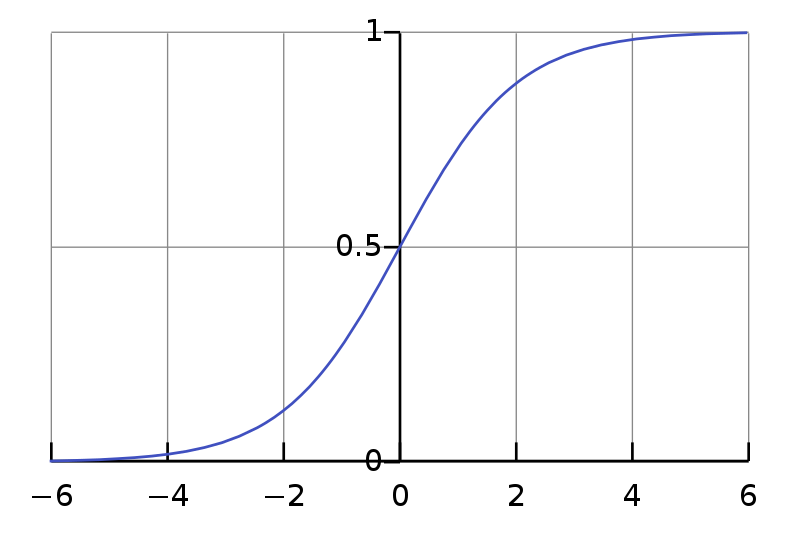
\includegraphics[scale = 0.15]{figs/logistic_curve}
	\end{figure}
\centering
	$$P(Y=1) = \text{logistic}(\beta_0+\beta_1 X)$$
	\medskip
	
	is equivalent to:
	\medskip
	
	$$\log(\text{Odds}(Y=1))=\beta_0+\beta_1 X$$
	
	


\end{frame}


\begin{frame}{
\includegraphics[scale = 0.015]{figs/technical} Another motivation for logistic regression}
	
	\vspace{-5 mm}

	\centering
	\[\text{logistic}(\beta_0+\beta_1X)=\frac{1}{1+e^{-(\beta_0+\beta_1X)}}\]
	so
	\[P(Y=1)=\frac{1}{1+e^{-(\beta_0+\beta_1X)}}\]
	
	\[\frac{P(Y=1)}{1-P(Y=1)}=e^{(\beta_0+\beta_1X)}\]
	
	\[\text{Odds}(Y=1)=e^{(\beta_0+\beta_1X)}\]
	
	\[\log(\text{Odds}(Y=1))=\log(e^{(\beta_0+\beta_1X)})\]
	
	\[\log(\text{Odds}(Y=1))=\beta_0+\beta_1X\]
	
\end{frame}

\begin{frame}{Logistic regression: fitting the model in \texttt{R}}
	The \texttt{lm} function won't do it for us anymore. Instead we use the \texttt{glm} function. 
	\\ ~\ 
	
	GLM stands for ``generalized linear model" and represents a whole class of regression methods. All you need to know is that \texttt{glm} syntax is a lot like \texttt{lm} syntax, but we must also specify $\texttt{family = binomial()}$ for logistic regression. Our command will look like
	\\ ~\
	
	\texttt{glm(y $\sim$ x, family = binomial(), data = dat)}
\end{frame}

\begin{frame}[fragile]{Simple logistic regression in \texttt{R}: HIV example}
	\vspace{-0.5cm}
	
	Let's fit our logistic regression model 
	\footnotesize
	
	\begin{verbatim}
		> mod <- glm(data = HIV, results ~ incentive, family = binomial())
		> summary(mod)
		
		Call:
		glm(formula = results ~ incentive, family = binomial(), data = HIV)
		
		Deviance Residuals: 
		Min       1Q   Median       3Q      Max  
		-1.7690  -0.9112   0.6851   0.6851   1.4693  
		
		Coefficients:
		Estimate Std. Error z value Pr(>|z|)    
		(Intercept) -0.66430    0.08473  -7.841 4.48e-15 ***
		incentive    1.99426    0.09961  20.022  < 2e-16 ***
		---
		Signif. codes:  0 ‘***’ 0.001 ‘**’ 0.01 ‘*’ 0.05 ‘.’ 0.1 ‘ ’ 1
	\end{verbatim}
	\normalsize
	
	\textcolor{violet}{Pollev:} Are the results on the log odds scale or the odds scale? 
	\tiny{\url{https://PollEv.com/multiple_choice_polls/sQteD6qdogbfQ7K2SVS1O/respond}}
	
	
\end{frame}

\begin{frame}[fragile]{Logistic regression}
	\vspace{-5 mm}
	
	As some estimates were negative, \textbf{\texttt{R} has given us the raw regression coefficient estimates and intervals on the log odds scale}. But the exponentiated versions are much more interpretable!
	\medskip
	\small
	\begin{verbatim}
	> exp(coef(mod))
	(Intercept)   incentive 
	0.5146341   7.3467940 
	
	> exp(confint(mod))
	Waiting for profiling to be done...
	2.5 %    97.5 %
	(Intercept) 0.4352074 0.6067626
	incentive   6.0516224 8.9432892
	\end{verbatim}
	\normalsize
	
	\medskip
	We can use \texttt{coef} to pull out coefficients, and then exponentiate (same for \texttt{confint}). 
	\\ ~\ 
	
	Note: The p-values for the hypothesis tests can be used directly since a test of $H_0: \beta_1 = 0$ is the same as a test of $H_0: \exp(\beta_1) = 1$. More on this next!
\end{frame}

\begin{frame}[fragile]{A note on confidence intervals and p-values}
	\vspace{-0.7cm}
	Here are our exponentiated confidence intervals:
	
		\begin{verbatim}
	> exp(confint(mod))
	Waiting for profiling to be done...
	2.5 %    97.5 %
	(Intercept) 0.4352074 0.6067626
	incentive   6.0516224 8.9432892
	\end{verbatim}
	For the \texttt{incentive} predictor, we have a point estimate of 7.34 with 95\% CI (6.05 8.94). It's a bit subtle, but this CI isn't actually symmetric about our point estimate!
	\medskip
	
	\begin{figure}
		\centering
		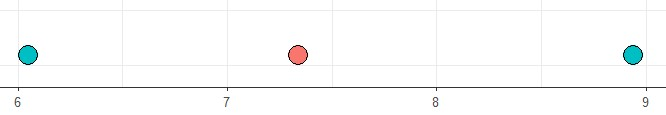
\includegraphics[scale = 0.4]{figs/confint}
	\end{figure}

\end{frame}

\begin{frame}{A note on confidence intervals and p-values}
	What's going on here? 
	\\ ~\
	
	\texttt{glm} is working on the log-odds scale:
	\begin{align*}
		&\text{Confidence interval: }(\hat{\beta} - 1.96 \times \hat{\text{SE}}, \hat{\beta} + 1.96 \times \hat{\text{SE}})\\
		&\text{Hypothesis test: }H_0: \beta = 0 \tab H_1: \beta \neq 0
	\end{align*}
	When you exponentiate to the odds scale, the interval is no longer symmetric and the hypotheses are different:
	\begin{align*}
		&\text{Confidence interval: }(e^{\hat{\beta} - 1.96 \times \hat{\text{SE}}}, e^{\hat{\beta} + 1.96 \times \hat{\text{SE}}})\\
		&\text{Hypothesis test: }H_0: \exp(\beta) = 1 \tab H_1: \exp(\beta) \neq 1
	\end{align*} 
	The p-values are unaffected (if the log-odds scale CI doesn't overlap 0, then the odds scale CI won't overlap 1)
\end{frame}
%
\subsection{Multiple logistic regression}
% interpretation: multiple/general, do the math
%%% beta 0


% interpretation: multiple/general, do the math
%%% beta 0
\begin{frame}
	\frametitle{Multiple logistic regression}
	
	\vspace{-5 mm}
	
	As with linear regression, we can have multiple predictors
	\medskip
	
	$$\log\left(\text{Odds}[Y =1 |X_1,\cdots,X_p]\right) = \beta_0 + \beta_1 X_1 + \beta_2X_2 + \cdots \beta_p X_p$$
	
	\medskip
	
	\textbf{In groups, try to interpret the following:}
	\medskip
	
	\begin{itemize}
		\item \textcolor{blue}{$\beta_0$}
		\medskip
		\item \textcolor{blue}{$\exp(\beta_0)$}
		\medskip
		\item \textcolor{blue}{$\beta_1$}
		\medskip
		\item \textcolor{blue}{$\exp(\beta_1)$}
	\end{itemize}
\end{frame}

\begin{frame}
	\frametitle{Multiple logistic regression}
	
	\vspace{-5 mm}
	
	As with linear regression, we can have multiple predictors
	\medskip
	
	$$\log\left(\text{Odds}[Y =1 |X_1,\cdots,X_p]\right) = \beta_0 + \beta_1 X_1 + \beta_2X_2 + \cdots \beta_p X_p$$
	
	\medskip
	
	\textbf{In groups, try to interpret the following:}
	\medskip
	
	\begin{itemize}
		\item \textcolor{blue}{$\beta_0$} : the log odds of $Y=1$ when all predictors are 0
		\medskip
		\item \textcolor{blue}{$\exp(\beta_0)$} : the odds of $Y=1$ when all predictors are 0
		\medskip
		
		\item \textcolor{blue}{$\beta_1$} : the log odds ratio comparing groups that differ by one unit of $X_1$ but have the same value for all other predictors
		
		\medskip
		\item \textcolor{blue}{$\exp(\beta_1)$} : the odds ratio of $Y=1$ comparing groups that differ by one unit of $X_1$ but have the same value for all other predictors
	\end{itemize}
\end{frame}


\begin{frame}{Example: HIV Test and Cash Incentives}
	Let's return to our study of choosing to receive an HIV test result and receiving an incentive.
	\\ ~\
	
	The \texttt{HIV} data has some other available information on the subjects in the study (not a full list):
	\medskip
	\begin{itemize}
		\item Incentive amount (USD)
		\item Age (years)
		\item Incentive (yes/no)
		\item Results (yes/no)
	\end{itemize}
\medskip  

	\textbf{We are interested in assessing the potential association between receiving an incentive and choosing to get HIV test results.} 
\end{frame}

\begin{frame}{Example: HIV Test and Cash Incentives}
	We will include age as another predictor.
	
	$$\log\left(\text{Odds}[\text{results} |\text{incentive, age}]\right) = \beta_0 + \beta_1 \text{incentive} + \beta_2\text{age}$$

\medskip

\textcolor{violet}{Pollev}: What is the interpretation of $\exp(\beta_0)$?
\bigskip

\textcolor{blue}{The odds of choosing to get a result among people of age 0 who did not get an incentive. (Doesn't make scientific sense)}
\bigskip


\textcolor{violet}{Pollev}: What is the interpretation of $\exp(\beta_1)$?
\bigskip

\textcolor{blue}{The odds ratio of choosing to get a result comparing two groups of the same age, one which received an incentive and one which did not.}

\end{frame}

\begin{frame}[fragile]{Example: HIV Test and Cash Incentives in \texttt{R}}
	
	\vspace{-8 mm}
	
\scriptsize
\begin{verbatim}
> mod <- lm(data = HIV, results ~ incentive + age)
> summary(mod)

Call:
lm(formula = results ~ incentive + age, data = HIV)

Residuals:
Min      1Q  Median      3Q     Max 
-0.8634 -0.3286  0.1978  0.2261  0.6887 

Coefficients:
Estimate Std. Error t value Pr(>|t|)    
(Intercept) 0.2893352  0.0252396  11.464  < 2e-16 ***
incentive   0.4485102  0.0191961  23.365  < 2e-16 ***
age         0.0015699  0.0005825   2.695  0.00708 ** 
---
Signif. codes:  0 ‘***’ 0.001 ‘**’ 0.01 ‘*’ 0.05 ‘.’ 0.1 ‘ ’ 1

Residual standard error: 0.422 on 2822 degrees of freedom
Multiple R-squared:  0.1658,	Adjusted R-squared:  0.1652 
F-statistic: 280.4 on 2 and 2822 DF,  p-value: < 2.2e-16

> exp(coefficients(mod))
(Intercept)   incentive         age 
1.335539    1.565977    1.001571
\end{verbatim}
\end{frame}

\begin{frame}{Logistic Regression with Categorical Variables}
	\textit{This content was added after we finished this chapter, in case anyone uses these notes as reference in the future.}
	\bigskip
	
	\textbf{Question:} How do we test the association between a categorical variable and a binary outcome with logistic regression?
	
	\bigskip
	
	\textbf{Answer:} We can again use the \texttt{anova} function.
	
	\bigskip
	
	\textcolor{blue}{$H_0$: \textbf{all} of the odds ratios comparing levels of the category to the reference level are equal to 1.}
	
	\bigskip
	
		\textcolor{blue}{$H_a$: \textbf{at least one} of the odds ratios comparing levels of the category to the reference level is not equal to 1.}
\end{frame}

\begin{frame}[fragile]{Logistic Regression with Categorical Variables}
	\vspace{-5 mm}
	
	Lets create an age category variable with categories "Under 20", ``20s and 30s", and ``40 and above".
	
	\scriptsize
	
	\begin{verbatim}
	HIV <- HIV %>% mutate(age_cat = 
	                        case_when(age < 20 ~ "Under 20",
	                                  age >= 20 & age < 40 ~ "20s and 30s",
	                                  age >= 40 ~ "40 and above"))
	
	mod <- glm(data = HIV, results ~ age_cat, family = binomial)
	mod_null <- glm(data = HIV, results ~ 1, family = binomial)
	
	anova(mod_null,mod,test = "LRT")
	Analysis of Deviance Table
	
	Model 1: results ~ 1
	Model 2: results ~ age_cat
	  Resid. Df Resid. Dev Df Deviance Pr(>Chi)  
	1      2824     3490.3                       
	2      2822     3481.9  2   8.4103  0.01492 *
	---
	Signif. codes:  0 ‘***’ 0.001 ‘**’ 0.01 ‘*’ 0.05 ‘.’ 0.1 ‘ ’ 1
	\end{verbatim}
	
	\normalsize
	At a 5\% significance level, we conclude there is an association between age category and odds of receiving a test result (p = 0.015).
	
	\medskip
	
	\textit{End of added content.}
	
\end{frame}

\subsection{Adjustment variables}

\begin{frame}{Logistic regression: formulating statistical question}


	
	\medskip
	
	\begin{enumerate}
		\item \textbf{Scientific Question:}  Is there an association between getting an incentive and choosing to go get HIV test results?
		
		\medskip
		
		\item \textbf{Statistical Question:} 
		\medskip
		  
		\begin{itemize}
			\item How is our outcome quantified? *The study is already completed -- we don't really have any control over this!* 
			
			\medskip
			
			\item[] \textcolor{blue}{Binary: getting results = 1, not getting results = 0} 
			
			\medskip
			
			\item How will we quantify association?  
			
			\medskip
			
			\item[] \textcolor{blue}{Ratio of odds of getting results comparing a group that received an incentive to a group that did not.} 
			
			\medskip
			
			\item Are there other variables we should adjust for? 
			
			\medskip
			
			\item[] \textcolor{blue}{Draw the causal diagram!} 
		\end{itemize}
	\end{enumerate}
\end{frame}

\begin{frame}{Causal diagram}
	\vspace{-5mm}
		
	\textbf{To talk about adjustment variables, lets pretend that incentives were not randomized but instead the nurse decided who received incentives. Test center location was still randomly assigned after incentive vouchers were given.}
	
\medskip
	
	Here's a reasonable causal diagram:
	\begin{center}
		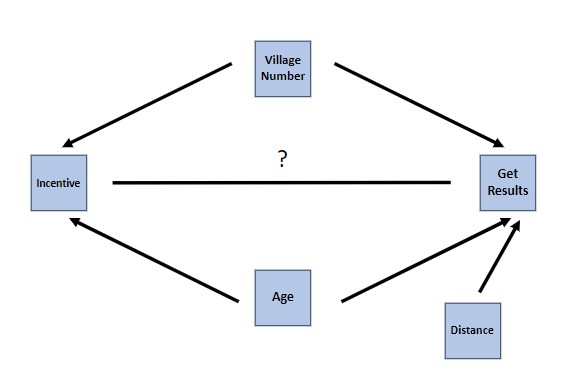
\includegraphics[scale = 0.55]{./figs/HIV_dag}
	\end{center}
	
\end{frame}


\begin{frame}{Logistic regression: Adjustment variable types}
	Previously, we discussed three types of variables we might include in a linear regression model in addition to the predictor of interest:
	\medskip
	\begin{itemize}
		\item \textcolor{blue}{Confounder}: Necessary to include in order to understand the association between predictor of interest and outcome
		
		
		\medskip
		
		\item \textcolor{blue}{Precision variable}: causally related to outcome but not associated with predictor of interest. Including in model increases precision
		
		\medskip
		
		\item \textcolor{blue}{Effect modifier}: association between predictor of interest and outcome varies by values of the effect modifier 
	\end{itemize}
\end{frame}

\begin{frame}{Logistic regression: Confounders}
	What do we do in logistic regression?
	\bigskip
	
	The good news is: \textcolor{blue}{The strategy of adjusting for confounders in our model has not changed!} We're just working on the log-odds scale now. 
	

\end{frame}


\begin{frame}{Logistic regression: Precision variables}
	Recall from our \textit{linear} regression unit that a precision variable $Z$ is 
	
	\medskip
	
	\begin{enumerate}
		\item Causally related to the outcome $Y$
		
	\medskip
		
		\item NOT associated with the predictor of interest $X$ 
	\end{enumerate}

\medskip

	Including $Z$ in our linear regression model increases the precision with which we can estimate the coefficient for $X$. 
	
	\bigskip
	
	\textbf{\textcolor{blue}{However, precision variables don't really exist in logistic regression.}} In some cases, adjusting for $Z$ in logistic regression can \textit{increase} our standard error on the coefficient for $X$. 

\end{frame}

\begin{frame}{Logistic regression: Interaction/effect modification}
	\vspace{-5 mm}
	
	Just as in (multiple) linear regression, we can include interaction terms in logistic regression to study effect modification. 
	
	\bigskip
	
	 If $X$ is our predictor of interest and $W$ our potential effect modifier: 
	\begin{align*}
	\log(\text{Odds}[Y = 1 \mid X, W]) = \beta_0 + \beta_1X + \beta_2W + \beta_3XW
	\end{align*} 
	
	\medskip
	
	In linear regression, interaction coefficients represent a difference of differences.
	
	\bigskip
	
	\textcolor{blue}{In logistic regression, interaction coefficients represent a (log) ratio of ratios.}
	
	
	\[\text{Odds}[Y = 1 \mid X, W] = e^{\beta_0}\times e^{\beta_1X}\times e^{\beta_2W} \times e^{\beta_3XW}\] 

\end{frame}

\begin{frame}{Logistic regression: Interaction/effect modification}
	\vspace{-5 mm}
	
	Suppose $W$ is binary. 
	
	\bigskip
	
	Difference in log-odds comparing groups \textcolor{blue}{differing by one unit} in $X$: 
	
	\bigskip
	
	\textcolor{blue}{When $W = 0$}:
	\begin{small}
		\begin{align*}
		&\log(\text{Odds}[Y = 1 \mid X = x+1, W = 0]) - \log(\text{Odds}[Y = 1 \mid X = x, W = 0])\\
		&= \Big\{\beta_0 + \beta_1(x + 1) + \beta_2\times 0 + \beta_3 \times 0 \Big\}- \Big\{\beta_0 + \beta_1(x) + \beta_2\times 0 + \beta_3 \times 0\Big\}\\
		&= \beta_1 
		\end{align*}
	\end{small} 



	\textcolor{blue}{When $W = 1$}::
	\begin{small}
		\begin{align*}
		&\log(\text{Odds}[Y = 1 \mid X = x+1, W = 1]) - \log(\text{Odds}[Y = 1 \mid X = x, W = 1])\\
		&= \Big\{\beta_0 + \beta_1(x + 1) + \beta_2\times 1 + \beta_3(x+1) \times 1 \Big\}\\
		&\tab - \Big\{\beta_0 + \beta_1(x) + \beta_2\times 1 + \beta_3 (x)\times 1\Big\}\\
		&= \beta_1 + \beta_3
		\end{align*}
	\end{small}
\end{frame}

\begin{frame}{Logistic regression: Interaction/effect modification}
	Interpreting what we saw on the previous slide:  
	
	\medskip
	
	\begin{itemize}
		\item $\beta_1$: Difference in log-odds comparing groups differing by one unit in $X$, among those with $W = 0$ 
		
		\medskip
		
		\item $\beta_1 + \beta_3$: Difference in log-odds comparing groups differing by one unit in $X$, among those with $W = 1$ 
	\end{itemize}

\bigskip

	So $\beta_3$ is the \textcolor{blue}{difference in differences} of log-odds for groups 1 unit apart in $X$, comparing the $W = 1$ group to the $W = 0$ group. 
	
	\bigskip
	
	\textcolor{blue}{This is exactly as in linear regression, just on the log-odds scale.}
\end{frame}

\begin{frame}{Logistic regression: Interaction/effect modification}
	
	Of course, log-odds aren't very interpretable. Exponentiating:
	
	\medskip
	
	\begin{itemize}
		\item $e^{\beta_1}$: Odds ratio comparing groups differing by one unit in $X$, among those with $W = 0$ 
		
		\medskip
		
		\item $e^{\beta_1 + \beta_3}$: Odds ratio comparing groups differing by one unit in $X$, among those with $W = 1$ 
	\end{itemize}

\bigskip

	Taking the ratio, we have
	\begin{align*}
	\frac{e^{\beta_1 + \beta_3}}{e^{\beta_1}} = \frac{e^{\beta_1}e^{\beta_3}}{e^{\beta_1}} = e^{\beta_3}
	\end{align*} 
	
	\medskip
	
	So, $e^{\beta_3}$ is the \textcolor{blue}{ratio of odds ratios} for groups 1 unit apart in $X$, comparing the $W = 1$ group to the $W = 0$ group. 
\end{frame}

\begin{frame}{Logistic regression: Interaction/effect modification}
	Summary: 
	
	\bigskip
	
	\begin{itemize}
		\item Fundamentally, interaction terms work the same in logistic regression as in linear regression, but on the log-odds scale
		
		\medskip
		
		\item Since we prefer to work directly with odds, the exponentiated interaction coefficient is the ratio of odds ratios for groups 1 unit apart in the predictor ($X$), comparing groups 1 unit apart in the effect modifier ($W$)
	\end{itemize}
\end{frame}




\begin{frame}{\textcolor{violet}{Pollev:} Interaction/effect modification example}
	
	\vspace{-5 mm}
	
	Question: Does whether someone is older than 50 years old might modify the association between incentives and getting HIV test results?
	
	
	\vspace{-3 mm}
	
	\color{blue}
	\begin{align*}
	\log(Odds&(\text{results}|\text{incentive, over\_50})) = \beta_0 + \beta_1\text{incentive}\\&+\beta_2\text{over\_50}+\beta_3\text{incentive}\cdot\text{over\_50}
	\end{align*}
	\color{black}
	
	\vspace{-2 mm}
	
	What is the expression for each of the following:
	
	\medskip
	
	\begin{itemize}
		\item Odds of getting a result among those who \textbf{don't} get an incentive and are \textbf{50 or younger}  \textcolor{purple}{\href{https://PollEv.com/multiple_choice_polls/1LE88Rsf2hnEYB0ktPIbl/respond}{link}}: \textcolor{blue}{$e^{\beta_0}$}
		
		\medskip
		
		\item Odds of getting a result among those who \textbf{don't} get an incentive and are \textbf{older than 50}  \textcolor{purple}{\href{https://PollEv.com/multiple_choice_polls/hSAtrOO3BuKbqy5zdGwch/respond}{link}}: \textcolor{blue}{$e^{(\beta_0+\beta_2)}$}
		
		\medskip
		
		\item Odds of getting a result among those who \textbf{do} get an incentive and are \textbf{50 or younger}  \textcolor{purple}{\href{https://PollEv.com/multiple_choice_polls/E513SDYKPbxFENUWdq6Ly/respond}{link}}:   \textcolor{blue}{$e^{(\beta_0+\beta_1)}$}
		
		\medskip
		
		\item Odds of getting a result among those who \textbf{do} get an incentive and are \textbf{older than 50} \textcolor{purple}{\href{https://PollEv.com/multiple_choice_polls/1L1S08HSw3G4P1isemgIt/respond}{link}}:  \textcolor{blue}{$e^{(\beta_0+\beta_1 + \beta_2 +\beta_3)}$}
		
		
		
	\end{itemize}
	
\end{frame}

\begin{frame}{\textcolor{violet}{Pollev:} Interaction/effect modification example}
	
	\vspace{-5 mm}
	
	\color{blue}
	\begin{align*}
	\log(Odds&(\text{results}|\text{incentive, over\_50})) = \beta_0 + \beta_1\text{incentive}\\&+\beta_2\text{over\_50}+\beta_3\text{incentive}\cdot\text{over\_50}
	\end{align*}
	\color{black}
	
	\vspace{-2 mm}
	
	What is the expression for each of the following:
	
	\medskip
	
	\begin{itemize}
		\item Odds ratio of getting a result \textbf{comparing those who do and do not} get an incentive, with \textbf{all 50 or younger} \textcolor{purple}{\href{https://PollEv.com/multiple_choice_polls/BTSCKv3ofieOMwW8bEYwT/respond}{link}}: \textcolor{blue}{$e^{\beta_1}$}
		
		\medskip
		
		\item Odds ratio of getting a result \textbf{comparing those are older than 50 and those who are at most 50}, with \textbf{all not getting an incentive} \textcolor{purple}{\href{https://PollEv.com/multiple_choice_polls/M9GzJr976YmfdwfTmqNUB/respond}{link}}:  \textcolor{blue}{$e^{\beta_2}$}
		
		\medskip
		
		\item Odds ratio of getting a result \textbf{comparing those who do and do not} get an incentive, with \textbf{all older than 50} \textcolor{purple}{\href{https://PollEv.com/multiple_choice_polls/QlJlfru1e0LWCDAjbmbHe/respond}{link}}: \textcolor{blue}{$e^{\beta_1+\beta_3}$}
		
		\medskip
		
		\item Odds ratio of getting a result \textbf{comparing those older than 50 and those who are at most 50}, with \textbf{all getting an incentive} \textcolor{purple}{\href{https://PollEv.com/multiple_choice_polls/uclSu0e57aLCbVT1ElIlw/respond}{link}}:   \textcolor{blue}{$e^{\beta_2+\beta_3}$}
		
		
		
	\end{itemize}
	
\end{frame}

\subsection{Reporting results}

\begin{frame}{Simple logistic regression: reporting results}
	\begin{enumerate}
		\item[4.] Perform \textit{statistical inference}:
		\begin{itemize}
			\item Calculate a test statistic
			\item Quantify uncertainty
			\item Perform hypothesis test
		\end{itemize}
		\item[5.] Add a conclusion
	\end{enumerate}

\medskip

	Based on logistic regression, we estimate that the odds of choosing to get an HIV test result are 7.35 times higher in subjects who receive an incentive versus those who do not. 
	
	\medskip
	
	Based on a 95\% confidence interval, the data would be consistent with a true odds ratio between 6.05 and 8.94. 
	
	\medskip
	
	Based on a test of the null hypothesis of an odds ratio of 1, there is sufficient evidence of an association between receiving an incentive and getting a test result (p $<$ 0.001). 
\end{frame}

\begin{frame}{Multiple logistic regression: reporting results}
	\vspace{-5mm}
	
	\begin{enumerate}
		\item[4.] Perform \textit{statistical inference}:
		\begin{itemize}
			\item Calculate a test statistic
			\item Quantify uncertainty
			\item Perform hypothesis test
		\end{itemize}
		\item[5.] Add a conclusion
	\end{enumerate}

\medskip
	
	Based on logistic regression, we estimate that the odds of choosing to get an HIV test result are 1.57 times higher in subjects who receive an incentive versus those who do not, comparing those of the same age. 
	
	\medskip
	
	Based on a 95\% confidence interval, the data would be consistent with a true odds ratio between 1.51 and 1.63. 
	
	\medskip
	
	Based on a test of the null hypothesis of an odds ratio of 1, there is sufficient evidence of an association between receiving an incentive and getting a test result (p = 0.007), after adjusting for age. 
\end{frame}

\begin{frame}{Effect modification: reporting results}
	\vspace{-5mm}
	
	\begin{enumerate}
		\item[4.] Perform \textit{statistical inference}:
		\begin{itemize}
			\item Calculate a test statistic
			\item Perform hypothesis test
		\end{itemize}
		\item[5.] Add a conclusion
	\end{enumerate}
	
	\medskip
	
	Based on logistic regression, we estimate that, among those 50 or younger, the odds of choosing to get an HIV test result are 1.57 times higher in subjects who receive an incentive versus those who do not. 
	
	\medskip
	
	We estimate that, among those over the age of 50, the odds of choosing to get an HIV test result are 1.53 times higher in subjects who receive an incentive versus those who do not. 
	
	\medskip
	
	Based on a test of the null hypothesis of a ratio of odds ratios of 1, there is insufficient evidence to reject the null that whether someone is over 50 does not modify the association between receiving an incentive and getting a test result (p = 0.67). 
\end{frame}

\begin{frame}{\textcolor{violet}{Pollev:} Adjustment Variable Review}
	
	\vspace{-5 mm}
	
	\textbf{To talk about adjustment variables, lets pretend that incentives were not randomized but instead the nurse decided who received incentives. Test center location was still randomly assigned after incentive vouchers were given.}
	
	
	\begin{figure}
		\centering
		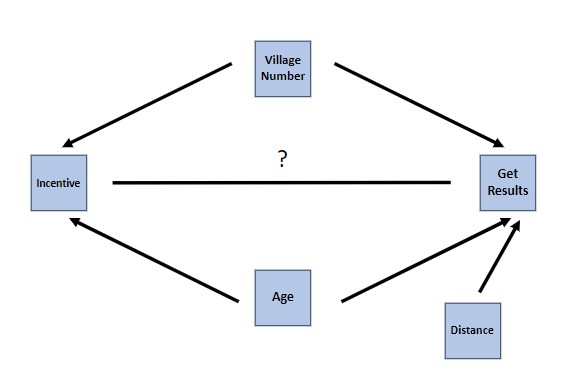
\includegraphics[scale = 0.35]{./figs/HIV_dag}
	\end{figure}
	
	Should we adjust for age? \textcolor{purple}{\href{https://PollEv.com/multiple_choice_polls/lzWdMlCQVpYspRIGYrxZF/respond}{link}} \textcolor{blue}{Yes, it is a potential confounder.}
	
	\medskip
	
	Should we adjust for distance? \textcolor{purple}{\href{https://PollEv.com/multiple_choice_polls/G6ujbX4n8V7eSjwyNysEe/respond}{link}} \textcolor{blue}{No, precision variables no longer exist for logistic regression.}
	
\end{frame}

%\begin{frame}{
\includegraphics[scale=0.01]{./figs/technical} Terminology}
%	You will often seen logistic regression framed a bit differently than what we've seen so far.  
%	\\ ~\ 
%	
%	You may see
%	\begin{align*}
%		\text{logit}(P[Y = 1 \mid X]) = \beta_0 + \beta_1 X
%	\end{align*}
%	where the logit function is defined as  
%	\begin{align*}
%		\text{logit}(p) = \log\Big(\underbrace{\frac{p}{1-p}}_{\text{odds}}\Big)
%	\end{align*}
%	 
%	Formally, the logit function is called a \textcolor{blue}{link} function, since it links our mean $E[Y \mid X] = P[Y = 1 \mid X]$ to our model $\beta_0 + \beta_1 X$. 
%\end{frame}

%

\subsection{Assumptions}

\begin{frame}{Assumptions for Logistic Regression}
	
	Assumptions are less straightforward for logistic regression then for linear regression. The two assumptions we will focus on are:
	
	\medskip
	
	\begin{itemize}
		
			\item \textcolor{blue}{Independence}: The errors $\epsilon_i$ are independent of each other
			
		
		\medskip
		
	\item \textcolor{blue}{Sample Size}: \textbf{Approximate Rule of Thumb}: There should be at least 10-20 events (the more rare outcome) per coefficient in the model
	\end{itemize} 

		

	
	
	
\end{frame}

\begin{frame}{Independence}
	
	\vspace{0.3cm}
	
	What does it \textit{mean} for this assumption to be violated?
	
	\vspace{0.3cm}
	
	\begin{itemize}
		\item[] Violating the independence assumption means that our observations are sampled in a way such that their responses are \textit{dependent}. Here are a few examples of when this might happen:
		\begin{itemize}
			\item We observe multiple individuals over time, and collect data on their outcomes at multiple time points. We expect the responses for a given individual to be \textit{dependent} over time (e.g. whether I am sick today \textit{depends} on whether I am sick tomorrow)
			\medskip
			\item We collect responses from individuals within groups. We expect people within the same group to (perhaps) score similarly, as they have things in common
		\end{itemize}
	\end{itemize}

\end{frame}

\begin{frame}{Independence in the HIV example}
	
	\textcolor{blue}{Question}: Is independence satisfied for the example of looking at the association between incentives and choosing to get a test result in the HIV data?
\end{frame}

%\begin{frame}[fragile]{Linearity}
%\vspace{-5 mm}
%	
%	\textcolor{blue}{Linearity is much trickier to assess for logistic regression than for linear regression.}
%	\bigskip
%	
%	However, one way we can attempt to assess linearity is plotting the residuals versus the fitted values on the log odds scale.
%	
%	\bigskip
%	
%	Standard residuals don't really make sense for logistic regression, so instead we use ``Pearson Residuals".
%	
%	\bigskip
%	
%	It only makes sense to assess linearity when we have at least one continuous predictor.
%	
%	\medskip
%	
%		\begin{verbatim}
%		library(car)
%	HIV2 <- HIV %>% filter(incentive != 0)
%	
%	mod <- glm(data = HIV2, results ~ amount, 
%	    family = binomial)
%	
%	residualPlot(mod)
%	
%	\end{verbatim}
%	
%
%	
%\end{frame}
%	
%	
%\begin{frame}{Linearity in HIV example}
%	
%
%
%\begin{figure}
%	\centering
%	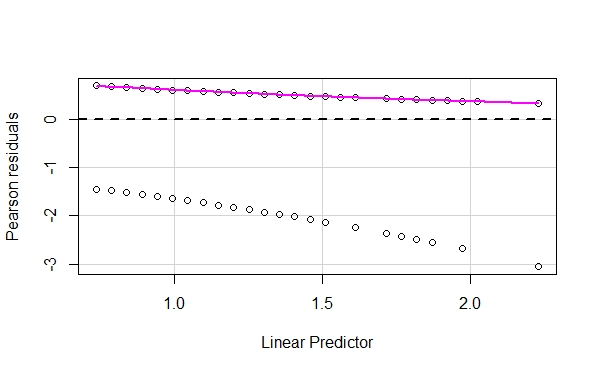
\includegraphics[scale = 0.6]{figs/resid_plot_HIV}
%\end{figure}
%
%
%\end{frame}	
%
%\begin{frame}[fragile]{Nonlinear Example}
%
%\begin{verbatim}
%library(car)
%
%x <- seq(-0.5,0.5,by = 0.01)
%
%logistic <- function(z){1/(1+exp(-z))}
%
%y <- rbinom(n = 101, size = 1, prob = logistic(3*x^2))
%
%mod <- glm(y ~ x, family = binomial)
%
%residualPlot(mod)
%\end{verbatim}
%
%\end{frame}
%
%\begin{frame}{Nonlinear Example}
%	
%	
%	\begin{figure}
%		\centering
%		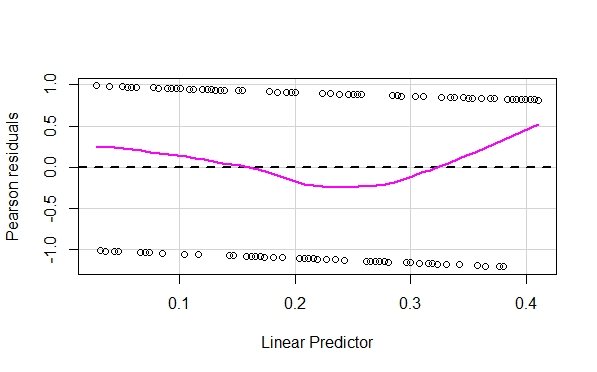
\includegraphics[scale = 0.6]{figs/resid_plot_nonlinear}
%	\end{figure}
%	
%	
%\end{frame}
%
%\begin{frame}[fragile]{Linear Example}
%	
%	\begin{verbatim}
%	library(car)
%	
%	x <- seq(-0.5,0.5,by = 0.01)
%	
%	logistic <- function(z){1/(1+exp(-z))}
%	
%	y <- rbinom(n = 101, size = 1, prob = logistic(x))
%	
%	mod <- glm(y ~ x, family = binomial)
%	
%	residualPlot(mod)
%	\end{verbatim}
%	
%\end{frame}
%
%\begin{frame}{Linear Example}
%	
%	
%	\begin{figure}
%		\centering
%		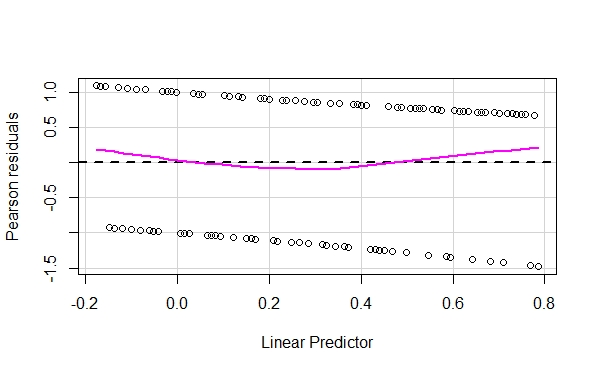
\includegraphics[scale = 0.6]{figs/resid_plot_linear}
%	\end{figure}
%	
%	
%\end{frame}


\section{Case-control studies}
%\begin{frame}
%	\frametitle{SECTION 4: CASE-CONTROL STUDIES}
%	% Learning objectives
%	By the end of this section, you should be able to:
%	\begin{itemize}
%		\item Describe why logistic regression is useful for the analysis of case-control data
%		\item Explain how and why logistic regression interpretation changes when we analyze case-control data
%	\end{itemize}
%\end{frame}

\begin{frame}{Recall: case-control study}
	\vspace{-5 mm}
	
	Description:
	\begin{itemize}
		\item \textit{Sample individuals based on the outcome} (some with, some without) and look back in time for exposure. 
	\end{itemize} 
\medskip
	Pros: 
	\begin{itemize}
		\item Efficient for rare outcomes 
		\item Cheaper and faster than cohort studies 
		\item Can study multiple exposures 
	\end{itemize}
	\medskip
	Cons: 
	\begin{itemize}
		\item In some scenarios, may not know time sequence of disease and exposure 
		\item \textcolor{red}{Cannot use to estimate relative risk or outcome prevalence} 
		\item Potential confounding (cannot make conclusions about causality)
	\end{itemize}
\end{frame}

\begin{frame}{Why can't we estimate RR or prevalence from case-control?}
	\textbf{In case-control studies, we cannot estimate relative risk or disease prevalence.}
	\\ ~\
	
	Why not? 
	\medskip
	
	\begin{itemize}
		\item This is a biased sampling scheme
		\medskip
		
		\item We do \textbf{not} have a representative sample of the population. We purposely sample more individuals who have the outcome ($Y = 1$) than we would 
		get from a simple random sample
		\medskip
			\begin{itemize}
				\item This is by design, and precisely why case-control studies are more efficient for rare outcomes!
			\end{itemize}
		
		\medskip
		
		\item Within categories $Y = 1$ (cases) and $Y = 0$ (controls), the samples should be representative but the overall sample is not
	\end{itemize} 
\end{frame}

\begin{frame}{Case-control sampling: Example}
	\vspace{-0.5cm}
	To illustrate this, consider the following \textcolor{blue}{population} of 1 million individuals:
	\begin{center}
		\begin{table}
			\begin{tabular}{|c|cc|c|}
				\hline 
				& Lung Cancer & No Lung Cancer &  \\ 
				& (Case) & (Control) & Total  \\
				\hline 
				Smoke & 900 & 4,100  & 5,000 \\ 
				No Smoke & 100 & 994,900 & 995,000  \\ 
				\hline 
				Total & 1000 & 999,000 & 1,000,000 \\ 
				\hline 
			\end{tabular}
		\end{table}
	\end{center} 
\medskip

	We are doing a case-control study on lung cancer and smoking. We have the resources to sample 400 individuals. We randomly pick 200 people with lung cancer and 200 without. Here's our \textcolor{blue}{sample}:
		\begin{center}
		\begin{table}
			\begin{tabular}{|c|cc|c|}
				\hline 
				& Lung Cancer & No Lung Cancer &  \\ 
				& (Case) & (Control) & Total  \\
				\hline 
				Smoke & 184 & 2  & 186 \\ 
				No Smoke & 16 & 198 & 214  \\ 
				\hline 
				Total & 200 & 200 & 400 \\ 
				\hline 
			\end{tabular}
		\end{table}
	\end{center}
\end{frame}

\begin{frame}{Case-control sampling: Example}
	\vspace{-0.3cm}
	\textcolor{blue}{Population:}
	\begin{center}
	\begin{table}
		\begin{tabular}{|c|cc|c|}
			\hline 
			& Lung Cancer & No Lung Cancer &  \\ 
			& (Case) & (Control) & Total  \\
			\hline 
			Smoke & 900 & 4,100  & 5,000 \\ 
			No Smoke & 100 & 994,900 & 995,000  \\ 
			\hline 
			Total & 1000 & 999,000 & 1,000,000 \\ 
			\hline 
		\end{tabular}
	\end{table}
\end{center} 
The prevalence of lung cancer in the \textcolor{blue}{population} is
\begin{align*}
	P^{\text{pop}}(\text{cancer}) = \frac{1,000}{1,000,000} = 0.001
\end{align*} 
The prevalence of lung cancer among people who do and do not smoke is
\begin{align*}
	&P^{\text{pop}}(\text{cancer} \mid \text{smoke}) = \frac{900}{5,000} = 0.18\\
	&P^{\text{pop}}(\text{cancer} \mid \text{no smoke}) = \frac{100}{995,000} = 0.0001
\end{align*}
\end{frame}

\begin{frame}{Case-control sampling: Example}
	\vspace{-0.3cm}
	\textcolor{blue}{Sample:}
		\begin{center}
	\begin{table}
		\begin{tabular}{|c|cc|c|}
			\hline 
			& Lung Cancer & No Lung Cancer &  \\ 
			& (Case) & (Control) & Total  \\
			\hline 
			Smoke & 184 & 2  & 186 \\ 
			No Smoke & 16 & 198 & 214  \\ 
			\hline 
			Total & 200 & 200 & 400 \\ 
			\hline 
		\end{tabular}
	\end{table}
\end{center} 
	The prevalence of lung cancer in the \textcolor{blue}{sample} is
	\begin{align*}
		P^{\text{samp}}(\text{cancer}) = \frac{200}{400} = 0.5 \tab \text{\textcolor{red}{(We chose this by design!)}}
	\end{align*} 
	The prevalence of lung cancer among people who do and do not smoke is
	\begin{align*}
		&P^{\text{samp}}(\text{cancer} \mid \text{smoke}) = \frac{184}{186} = 0.989\\
		&P^{\text{samp}}(\text{cancer} \mid \text{no smoke}) = \frac{16}{214} = 0.075
	\end{align*}
\end{frame}

\begin{frame}{Case-control sampling: Example}
	\vspace{-1cm}
	\begin{align*}
		P^{\text{pop}}(\text{cancer}) = 0.001 \tab \text{vs.} \tab P^{\text{samp}}(\text{cancer}) = 0.5
	\end{align*}
	Clearly, our sample estimate of the prevalence of lung cancer is not even close to the true prevalence -- we chose half our sample to be cases, so the 0.5 was completely determined by us.
	\\ ~\
	
	Similarly, our prevalence estimates separated by exposure are way off:
	\begin{small} 
	\begin{align*}
		&P^{\text{pop}}(\text{cancer} \mid \text{smoke}) = 0.18 \hspace{0.5cm} \text{vs.} \hspace{0.5cm} P^{\text{samp}}(\text{cancer}\mid \text{smoke}) = 0.989\\
		&P^{\text{pop}}(\text{cancer}\mid \text{no smoke}) = 0.0001 \hspace{0.2cm} \text{vs.} \hspace{0.2cm} P^{\text{samp}}(\text{cancer}\mid \text{no smoke}) = 0.075
	\end{align*}
	\end{small}
	Because we \textcolor{blue}{oversampled} cases, both exposed and unexposed subjects appear to be at much higher risk of cancer than they actually are. 
\end{frame}

\begin{frame}{Case-control sampling: Example}
	\small
	\vspace{-0.7cm}
	What about the prevalence of smoking among those with and without lung cancer? \textcolor{red}{Because we randomly sampled within cases and within controls, we can estimate these!}
	\\ ~\
	
	\textbf{Exercise:} In both the population and the sample, calculate the prevalence of smoking among cases and controls.
	\\ ~\
	
	\textcolor{blue}{Population:} 
	\begin{center}
		\begin{table}
			\begin{tabular}{|c|cc|c|}
				\hline 
				& Lung Cancer & No Lung Cancer &  \\ 
				& (Case) & (Control) & Total  \\
				\hline 
				Smoke & 900 & 4,100  & 5,000 \\ 
				No Smoke & 100 & 994,900 & 995,000  \\ 
				\hline 
				Total & 1000 & 999,000 & 1,000,000 \\ 
				\hline 
			\end{tabular}
		\end{table}
	\end{center}

\textcolor{violet}{Pollev:} What ratio of cases to controls would give us the same risks (asymptotically) in the exposed and unexposed as in the true population? \textcolor{purple}{\href{https://PollEv.com/multiple_choice_polls/AS3rMDos8Yz37Ba4eIv73/respond}{link}} \textcolor{blue}{1:999}

\end{frame}


\begin{frame}{Case-control sampling: Example}
	\small
	\vspace{-0.7cm}
	What about the prevalence of smoking among those with and without lung cancer? \textcolor{red}{Because we randomly sampled within cases and within controls, we can estimate these!}
	\\ ~\
	
	\textbf{Exercise:} In both the population and the sample, calculate the prevalence of smoking among cases and controls.
	\\ ~\

	\textcolor{blue}{Population:} 
		\begin{center}
		\begin{table}
			\begin{tabular}{|c|cc|c|}
				\hline 
				& Lung Cancer & No Lung Cancer &  \\ 
				& (Case) & (Control) & Total  \\
				\hline 
				Smoke & 900 & 4,100  & 5,000 \\ 
				No Smoke & 100 & 994,900 & 995,000  \\ 
				\hline 
				Total & 1000 & 999,000 & 1,000,000 \\ 
				\hline 
			\end{tabular}
		\end{table}
	\end{center}
 \textcolor{blue}{Sample}:
	\begin{center}
		\begin{table}
			\begin{tabular}{|c|cc|c|}
				\hline 
				& Lung Cancer & No Lung Cancer &  \\ 
				& (Case) & (Control) & Total  \\
				\hline 
				Smoke & 184 & 2  & 186 \\ 
				No Smoke & 16 & 198 & 214  \\ 
				\hline 
				Total & 200 & 200 & 400 \\ 
				\hline 
			\end{tabular}
		\end{table}
	\end{center}
\end{frame}

\begin{frame}{Case-control sampling: Example}
	\begin{align*}
		&P^{\text{pop}}(\text{smoke} \mid \text{cancer}) = \frac{900}{1,000} = 0.9\\
		&P^{\text{pop}}(\text{smoke} \mid \text{no cancer}) = \frac{4,100}{999,000} = 0.004\\
		&P^{\text{samp}}(\text{smoke} \mid \text{cancer}) = \frac{184}{200} = 0.92\\
		&P^{\text{samp}}(\text{smoke} \mid \text{no cancer}) = \frac{2}{200} = 0.01
	\end{align*}
	Although the numbers aren't identical due to sampling variability, the sample can be used to estimate these two probabilities. 
\end{frame}

\begin{frame}{Association between smoking and cancer}
	\vspace{-0.5cm}
	How do we measure association between two binary variables?  
	\begin{itemize}
		\item RD = $P$(cancer $\mid$ smoke) -  $P$(cancer $\mid$ no smoke) 
		\item RR = $P$(cancer $\mid$ smoke) $/$ $P$(cancer $\mid$ no smoke)
	\end{itemize}
	We can't estimate any of these probabilities from a case-control study.  
	\\ ~\
	
	What about the OR?
	\begin{itemize}
		\item OR = $\frac{P(\text{cancer} \mid \text{smoke})}{1 - P(\text{cancer} \mid \text{smoke})} / \frac{P(\text{cancer} \mid \text{no smoke})}{1 - P(\text{cancer} \mid \text{no smoke})}$
	\end{itemize}
	\vspace{0.2cm} 
	Seems like we're still out of luck. But what about the \textcolor{blue}{odds ratio for smoking comparing those with and without cancer?}
	\begin{itemize}
		\item $\text{OR}^* = \frac{P(\text{smoke} \mid \text{cancer})}{1 - P(\text{smoke} \mid \text{cancer})} / \frac{P(\text{smoke} \mid \text{no cancer})}{1 - P(\text{smoke} \mid \text{no cancer})}$
	\end{itemize}
	\vspace{0.2cm} 
	This doesn't really answer our scientific question...but doing a bit of math shows us an interesting relationship between OR and OR$^*$: \textbf{they're identical}!
\end{frame}

\begin{frame}{
\includegraphics[scale=0.01]{./figs/technical} Symmetry of the odds ratio}
	Let $D$ denote disease and $E$ exposure, with $\bar{D}$ and $\bar{E}$ meaning ``no disease" and ``no exposure," respectively. It turns out that 
	\begin{align*}
		\text{OR} = \frac{\frac{P(D \mid E)}{1 - P(D \mid  E)}}{\frac{P(D \mid \bar{E})}{1 - P(D \mid \bar{E})}} = \frac{\frac{P(E \mid D)P(D)}{P(E \mid \bar{D})P(\bar{D})}}{\frac{P(\bar{E} \mid D)P(D)}{P(\bar{E} \mid \bar{D})P(\bar{D})}} = \frac{\frac{P(E \mid D)}{P(\bar{E} \mid D)}}{\frac{P(E \mid \bar{D})}{P(\bar{E} \mid \bar{D})}} = \frac{\frac{P(E \mid D)}{1 - P(E \mid D)}}{\frac{P(E\mid \bar{D})}{1 - P(E\mid \bar{D})}} = \text{OR}^*
	\end{align*}
	The key to this relationship is \textcolor{blue}{Bayes' rule}. Ask if you're interested!
\end{frame}

\begin{frame}{Symmetry of the odds ratio: Example}
	\vspace{-0.8cm}
	Looking back at our example, we can see that the OR of cancer comparing people who do and do not smoke is identical to the OR of smoking comparing those with and without cancer. 
	\begin{center}
		\begin{table}
			\begin{tabular}{|c|cc|c|}
				\hline 
				& Lung Cancer & No Lung Cancer &  \\ 
				& (Case) & (Control) & Total  \\
				\hline 
				Smoke & 184 & 2  & 186 \\ 
				No Smoke & 16 & 198 & 214  \\ 
				\hline 
				Total & 200 & 200 & 400 \\ 
				\hline 
			\end{tabular}
		\end{table} 
	\end{center}
	\begin{align*}
		\text{OR} = \frac{\frac{P(\text{cancer} \mid \text{smoke})}{1 - P(\text{cancer} \mid \text{smoke})}}{\frac{P(\text{cancer} \mid \text{no smoke})}{1 - P(\text{cancer} \mid \text{no smoke})}}  = \frac{\frac{184}{2}}{\frac{16}{198}} = \frac{184\times 198}{16 \times 2} = 1138.5\\  
		\text{OR}^* =\frac{\frac{P(\text{smoke} \mid \text{cancer})}{1 - P(\text{smoke} \mid \text{cancer})}}{\frac{P(\text{smoke} \mid \text{no cancer})}{1 - P(\text{smoke} \mid \text{no cancer})}}  = \frac{\frac{184}{16}}{\frac{2}{198}} = \frac{184\times 198}{16 \times 2} = 1138.5
	\end{align*}
\vfill 
\tiny Note: We made up the numbers for this example! This odds ratio exaggerates the true association.

\end{frame}

\begin{frame}{Logistic regression in case-control studies}
	As we've seen, logistic regression allows us to estimate the odds ratio -- this is exactly what we want in a case-control study! But we still need to be careful.  
	\begin{align*}
		\log(\text{odds}[\text{cancer} \mid \text{smoke}]) = \beta_0 + \beta_1 \text{smoke}
	\end{align*} 
	\vspace{-3 mm}
	
	\begin{itemize}
		\item \sout{$e^{\beta_0}$: odds of cancer among people who do not smoke}
	\medskip
	
	\begin{itemize}
		\item  \normalsize odds[cancer $\mid$ no smoke] = $\frac{P(\text{cancer} \mid \text{no smoke})}{1 - P(\text{cancer} \mid \text{no smoke})}$
		
		\smallskip
		
		\item \normalsize Remember: our estimate of $P(\text{cancer} \mid \text{no smoke})$ is biased!
		 
		\smallskip
		
		\item \normalsize \textbf{In a case-control study, the intercept $\beta_0$ is not interpretable.} 
		
		\smallskip
		
		\item \normalsize	This won't stop \texttt{R} from giving you an intercept estimate anyway! It's up to you to interpret things correctly.
		\end{itemize}
	\end{itemize}
\end{frame}

\begin{frame}{Logistic regression in case-control studies}
	As we've seen, logistic regression allows us to estimate the odds ratio -- this is exactly what we want in a case-control study! But we still need to be careful. 
	\begin{align*}
		\log(\text{odds}[\text{cancer} \mid \text{smoke}]) = \beta_0 + \beta_1 \text{smoke}
	\end{align*}
	
	\vspace{-3 mm}
	
	\begin{itemize}
		
	\item $e^{\beta_1}$: odds ratio for cancer comparing people who do and do not smoke
	\medskip
	
	\begin{itemize}
		\item \normalsize This \textit{is} interpretable because it's mathematically equivalent to the odds ratio for smoking comparing those with and without cancer, which we can estimate. 
	\end{itemize}
	\end{itemize}
\end{frame}

\begin{frame}{Case-control studies: summary}
	Case-control studies involve biased sampling, which can be useful with a rare outcome. 
	\\ ~\ 
	
	We \textit{cannot} estimate
	\begin{itemize}
		\item Risk difference 
		\item Relative risk
	\end{itemize}
	\vspace{0.2cm}
	We \textit{can} estimate
	\begin{itemize}
		\item Odds ratio (via logistic regression)
		\item[] \tab \dots but remember that we cannot interpret the intercept
	\end{itemize}
	\vspace{0.2cm}
	This is a big reason for logistic regression's popularity in public health.  
\end{frame}

\section{Prediction}
\begin{frame}[fragile]{Logistic regression: Prediction}
\vspace{-5 mm}	
	
	We can also use logistic regression for prediction, though it takes a bit more work to get results on the scale we want. 
	\\ ~\
	
	Let's start with the a single quantitative predictor, incentive amount:
	\begin{align*}
		\log(\text{Odds}(\texttt{Results} \mid \texttt{Amount})) = \beta_0 + \beta_1 \texttt{Amount}
	\end{align*}
	\begin{center}
		\footnotesize
\begin{verbatim}
> HIV2 <- HIV %>% filter(incentive != 0)
> mod <- glm(data = HIV2, results ~ amount, family = binomial)
> summary(mod)

Call:
glm(formula = results ~ amount, family = binomial, data = HIV2)

Coefficients:
Estimate Std. Error z value Pr(>|z|)    
(Intercept)  0.68303    0.09319   7.329 2.32e-13 ***
amount       0.54629    0.07067   7.731 1.07e-14 ***
---
Signif. codes:  0 ‘***’ 0.001 ‘**’ 0.01 ‘*’ 0.05 ‘.’ 0.1 ‘ ’ 1
\end{verbatim}
\end{center}
\end{frame}

\begin{frame}{Logistic regression: Prediction}
	\vspace{-1cm}
			\begin{align*}
		\log(\text{Odds}(\texttt{Results} \mid \texttt{Amount})) = \beta_0 + \beta_1 \texttt{Amount}
		\end{align*}
	Let's predict for a person who receives a \$2 incentive:
	\begin{enumerate}
		\item Get estimates for each regression coefficient: 
		\item[] $\hat{\beta}_0 = 0.683, \hat{\beta}_1 = 0.546$
		\item Plug in estimates and predictor values:
		\begin{enumerate}
			\item[a.] $\widehat{\log(\text{Odds})} = 0.683 + (0.546\times2$) = 1.775
			\item[b.] $\widehat{\text{Odds}} = e^{1.775} = 5.900$
			\item[] \textcolor{blue}{(using that $e^{\log x} = x$)}
			\item[c.] $\widehat{\text{Prob}} = \frac{5.9}{1 + 5.9} = 0.855$
			\item[] \textcolor{blue}{(using that Odds = $\frac{\text{Prob}}{1-\text{Prob}}$ and so Prob = $\frac{\text{Odds}}{1  +\text{Odds}}$)}
		\end{enumerate}
	\end{enumerate}
\smallskip
	There's a common shortcut to get from \textcolor{blue}{a.} to our final answer. 
	\begin{align*}
		\text{expit}(x) = \frac{e^x}{1 + e^x} \Rightarrow \text{expit}(1.775) = 0.855
	\end{align*}
\end{frame}

\begin{frame}[fragile]{Logistic regression: Prediction}
	\vspace{-5mm}
	
	Of course, \texttt{R} will do all the work for us: 
	
	\small
	\begin{verbatim}
	> predict(mod, newdata = data.frame(amount = 2))
	1 
	1.775613
	
	> predict(mod, newdata = data.frame(amount = 2), 
	    type = "response")
	1 
	0.8551543 
	\end{verbatim}
	
	\medskip
	
	\normalsize
	We need to use \texttt{type = "response"} to predict on the probability scale

\bigskip

	Unlike linear regression, logistic regression keeps all fitted and predicted values in [0,1]
	
	
\end{frame}


\begin{frame}{Prediction for binary outcomes}
	
	\vspace{-5 mm}
	
	For quantitative outcomes, we discussed predictive accuracy in terms of \textcolor{blue}{$R^2$} (using the training data) and \textcolor{blue}{MSE} (using the test data).  
	\\ ~\
	
	Neither of these metrics makes much sense for predicting binary outcomes, where we want to be able to say whether an individual is a 0 or a 1 based on their covariate values.  
	\\ ~\
	
	What's more, logistic regression gives us predictions on a probability scale, not a binary scale.  
	\\ ~\
	
	Two unsettled questions: 
	\begin{enumerate}
		\item How do we turn predictions on probability scale into binary predictions?  
		\item How do we evaluate the quality of these predictions? 
	\end{enumerate}

\bigskip

\textcolor{violet}{Pollev: \href{https://PollEv.com/multiple_choice_polls/RrcDDezBoaDcZesDbQOdt/respond}{link} } Can we use case control data to make predictions? \pause\textcolor{blue}{No.}

\end{frame}


\begin{frame}{Binary predictions}
	We fit the model
	\begin{align*}
		\log(\text{Odds}(Y = 1 \mid X_1, \dots, X_p)) = \beta_0 + \beta_1X_1 + \cdots + \beta_pX_p
	\end{align*} 
	Using our estimated coefficients, we get a probability prediction
	\begin{align*}
		\widehat{P}(Y = 1 \mid X_1, \dots, X_p) = \text{expit}(\hat{\beta}_0 + \hat{\beta}_1X_1 + \cdots + \hat{\beta}_pX_p)
	\end{align*} 
	$\hat{P}$ is a number in (0,1). We want to predict whether $Y = 1$ or $Y = 0$ based on $X_1,\dots, X_p$. 
	\\ ~\ 
	
	\textbf{Question:} What are some ideas for turning a probability prediction into a binary prediction? 
	\\ ~\  
	
	\textbf{Answer:} Choose a threshold and assign 1 to all predicted values above the threshold, and 0 to all below. 
\end{frame}

\begin{frame}{Binary predictions}
	Our procedure for binarizing predictions: 
	\medskip
	\begin{enumerate}
		\item Pick a cutoff $c$ between 0 and 1. 
		\medskip
		
		\item For each individual $i$ in the test set, generate a probability prediction 
		\begin{align*}
			\widehat{P}(Y_i = 1 \mid X_{i,1}, \dots, X_{i,p}) = \text{expit}(\hat{\beta}_0 + \hat{\beta}_1X_{i,1} + \cdots + \hat{\beta}_pX_{i,p})
		\end{align*}  
		\item Given a prediction $\hat{P}_i$, generate a binary prediction $\hat{Y}_i$ by declaring this individual a 1 if $\hat{P}_i> c$, and 0 otherwise.  
	\end{enumerate}
\medskip
	So, now that we've got binary predictions, let's see how we did. 
\end{frame}

\begin{frame}{Sensitivity and specificity}
	You may remember \textcolor{blue}{sensitivity} and \textcolor{blue}{specificity} from BIOST 310, in the context of testing for a disease. We'll be a bit more general here.  
	
	\medskip
	\begin{itemize}
		\item \textcolor{blue}{Sensitivity}: the probability that $\hat{Y} = 1$ given that $Y = 1$, or $P(\hat{Y}= 1 \mid Y = 1)$. Sometimes called the ``true positive rate" 
		
		\medskip
		\item \textcolor{blue}{Specificity}: the probability that $\hat{Y}= 0$ given that $Y = 0$, or $P(\hat{Y} = 0 \mid Y = 0)$. $1 - $specificity is sometimes called the ``false positive rate"$^*$ 
	\end{itemize}
	
\medskip
 $^*$This is because $1 - P(\hat{Y}= 0 \mid Y = 0) = P(\hat{Y}= 1 \mid Y = 0)$, which is the probability of a false positive. 
\end{frame}

\begin{frame}{Sensitivity and specificity}
	How do we estimate these quantities? 
	
	\medskip
	
	\begin{itemize}
		\item \textcolor{blue}{Sensitivity}: $\frac{\text{\# of individuals with }\hat{Y}= 1 \text{ and } Y = 1}{\text{\# of individuals with }Y = 1}$ 
		
		\medskip
		
		\item \textcolor{blue}{Specificity}: $\frac{\text{\# of individuals with }\hat{Y}= 0 \text{ and } Y = 0}{\text{\# of individuals with }Y = 0}$ 
	\end{itemize}
\end{frame}

\begin{frame}{Sensitivity and specificity}
	
	\vspace{-7 mm}
	
	How are sensitivity and specificity affected by our choice of cutoff $c$?   
	\smallskip
	
	(Remember: $\hat{P}$ = estimated probability of $Y = 1$ given covariates.)
	
	\medskip
	
	\begin{itemize}
		\item $c = 0$: Since $\hat{P} > 0$ for all individuals, we classify everyone as 1 
		
		\smallskip
		
		\item $c = 1$: Since $\hat{P} < 1$ for all individuals, we classify everyone as 0 
		
		\smallskip
		
		\item $0 < c < 1$: Something in the middle  
	\end{itemize}

	\medskip

	\textbf{Key point:} \textcolor{blue}{As we increase $c$, we (1) increase specificity and (2) decrease sensitivity}  
	
	\medskip
	\begin{itemize}
		\item Higher $c$ means:  
		\smallskip
		
		\begin{itemize}
			\item fewer individiuals classified as 1 
			\item true number of individuals with $Y = 1$ doesn't change
			\item so sensitivity $P(\hat{Y}= 1 \mid Y = 1)$ goes down  
			
			\medskip
			\item more individuals classified as 0 
			\item true number of individuals with $Y = 0$ doesn't change
			\item so specificity $P(\hat{Y}= 0 \mid Y = 0)$ goes up
		\end{itemize}
	\end{itemize}
\end{frame}

\begin{frame}[fragile]{Sensitivity and specificity in \texttt{R}}
	
	\vspace{-7 mm}
	
	Back to our predictions of choosing to get HIV test results based on incentive amount!
	
	\bigskip
	
	\textbf{\textcolor{blue}{We need to split the data into training and testing sets.}}
	
	\textcolor{violet}{Pollev: \href{https://PollEv.com/multiple_choice_polls/5IQzGAIwsCTstq8ZYMssj/respond}{link}} Why? \pause \textcolor{blue}{to prevent overfitting!}
	
	\bigskip
	
	\footnotesize
	\begin{verbatim}
	HIV2 <- HIV %>% filter(incentive != 0)
	
	set.seed(32)
	test_set <- rep(0,nrow(HIV2))
	test_set[1:round(nrow(HIV2)*0.3)] <- 1
	
	test_set <- sample(test_set)
	
	train_data <- HIV2 %>% mutate(test = test_set) %>% filter(test == 0)
	test_data <- HIV2 %>% mutate(test = test_set) %>% filter(test == 1)
	
	mod <- glm(data = train_data, results ~ amount, family = binomial)
	
	test_data <- test_data %>% 
	  mutate(predictions = 
	           predict(mod, newdata = test_data, type = "response"))
	
	\end{verbatim}
	
\end{frame}

\begin{frame}[fragile]{Sensitivity and specificity in \texttt{R}}
	
	\vspace{-7 mm}
	
	Back to our predictions of choosing to get HIV test results based on incentive amount!
	
	\bigskip
	
	Let's take $c =0.5$. This is a sensible place to start --- if we predict someone has a greater than 50\% chance of choosing to get a result, we classify them as a case. 
	
	\footnotesize
	\begin{verbatim}	
	test_data %>% summarize(Sensitivity = 
	                          sum(predictions > 0.5 & results == 1)/
	                          sum(results == 1),
	                        Specificity = 
	                          sum(predictions <= 0.5 & results == 0)/
	                          sum(results == 0))
	                          
	 Sensitivity Specificity
	           1           0
	\end{verbatim}

\end{frame}

\begin{frame}{Sensitivity and specificity in \texttt{R}}
	\vspace{-0.5cm}
	Taking a look at our predictions, it's clear why we got these numbers...
			\begin{center}
		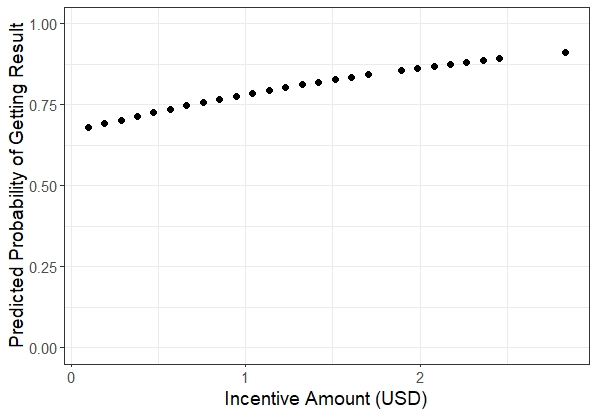
\includegraphics[scale = 0.5]{figs/hiv_prediction_plot}
	\end{center}
	No one had a predicted probability under 0.5, so we classified everyone as \texttt{results }$ = 1$. (Everyone in this subset received an incentive)
\end{frame}

\begin{frame}{ROC curve}
	Choosing a single cutoff $c$ doesn't give us a very good idea of the predictive performance of our logistic regression model. 
	\\ ~\
	
	What if we looked at the sensitivity and specificity of our predictive model as we vary $c$ between 0 and 1? 
	\\ ~\ 
	
	Plotting sensitivity (true positive rate) vs. $1-$specificity (false positive rate) gives the \textcolor{blue}{receiver operating characteristic (ROC) curve}. 
\end{frame}

\begin{frame}{ROC curve}
	\vspace{-0.3cm}
	\begin{center}
	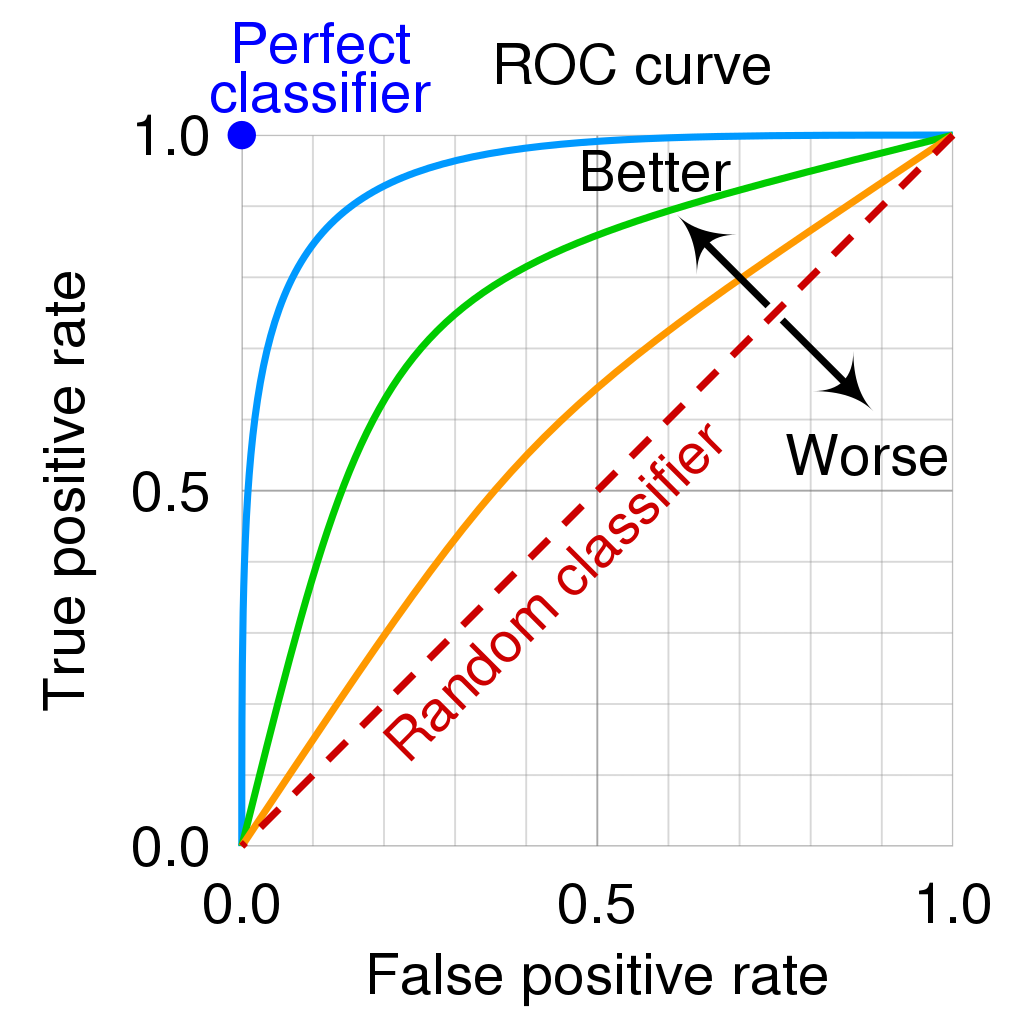
\includegraphics[width=0.7\textwidth]{./figs/roc_curve_example}
	\end{center}
\end{frame}

\begin{frame}{ROC curves}
	
	\vspace{-5 mm}
	
	What you should know about ROC curves:
	
	\medskip
	\begin{itemize}
		\item A curve passing through the top left corner indicates a perfect binary prediction model --- this says you can achieve a sensitivity and specificity of 1. (Of course, this never happens in practice) 
		
		\medskip
		 
		\item The diagonal represents a random prediction model (a coin flip)  
		
		\medskip
		
		\item The closer an ROC curve comes to the upper left corner, the better the prediction model
	\end{itemize}

\medskip

	By taking the \textcolor{blue}{area under the ROC curve}, we can get a single number telling us how well we've done. This is called the \textcolor{blue}{AUC}.  
	
	\medskip
	
	\begin{itemize}
		\item AUC of 1 is perfect 
		
		\smallskip
		\item AUC of 0.5 is a completely random model (coin flip)
		
		\medskip
		
		\item AUC $<0.5$ means you probably shouldn't use your prediction model --- you'd be better off flipping a coin
	\end{itemize}
\end{frame}

\begin{frame}{\textcolor{violet}{Pollev:} ROC curves}
	
	\vspace{-7 mm}
	
	\begin{center}
	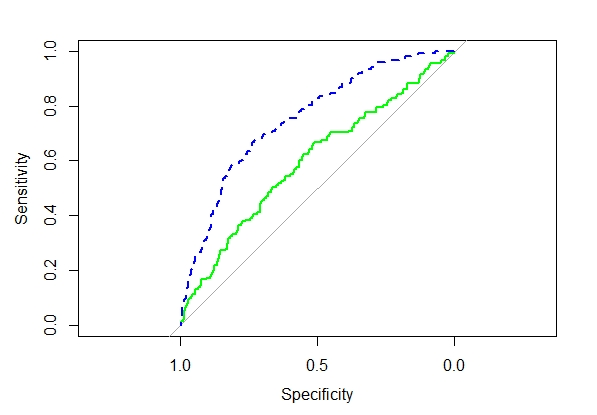
\includegraphics[scale = 0.6]{figs/roc_question}
\end{center}	

	\textcolor{violet}{\href{https://PollEv.com/multiple_choice_polls/bPijp7LawjdacrRp7AfVW/respond}{link}} Which model is better? \pause\textcolor{blue}{Blue dotted line}
\end{frame}


\begin{frame}{\textcolor{violet}{Pollev:} ROC curves}
	
	\textcolor{violet}{\href{https://PollEv.com/multiple_choice_polls/Mk1x5GCgquXHf2TBw8cFf/respond}{link}} Which model is best?
	
	\bigskip
	
	\begin{enumerate}
		\item Model A: AUC of 0.6
		\medskip
		\item Model B: AUC of 0.4
		\medskip
		\item Model C: AUC of 0.9
		\medskip
		\item  Model D: AUC of 0.7
	\end{enumerate}
\pause
	\bigskip
	\textbf{\textcolor{blue}{Model C}}
\end{frame}

\begin{frame}{\textcolor{violet}{Pollev:} ROC curves}
	
	\textcolor{violet}{\href{https://PollEv.com/multiple_choice_polls/2v8nB4YNfYWJKa2Hwzq2h/respond}{link}} Which model is worse than a coin flip?
	
	\bigskip
	
	\begin{enumerate}
		\item Model A: AUC of 0.6
		\medskip
		\item Model B: AUC of 0.4
		\medskip
		\item Model C: AUC of 0.9
		\medskip
		\item  Model D: AUC of 0.7
	\end{enumerate}
	\pause
	\bigskip
	\textbf{\textcolor{blue}{Model B}}
\end{frame}


\begin{frame}[fragile]{ROC curves in \texttt{R}}
	\vspace{-0.7cm}
	You could make an ROC curve ``by hand" in \texttt{R}, but we'll use the \texttt{pROC} package
	
	\medskip
	\footnotesize
	\begin{verbatim}
	library(pROC)
	
	roc(test_data %>% pull(results),
	    test_data %>% pull(predictions),
	    #arguments for plot
	    plot = TRUE,
	    auc.polygon = TRUE,
	    max.auc.polygon = TRUE,
	    grid = TRUE,
	    print.auc = TRUE)  
	  	\end{verbatim}
	  	
	  	\vspace{-6 mm}
	  	
	\begin{center}
	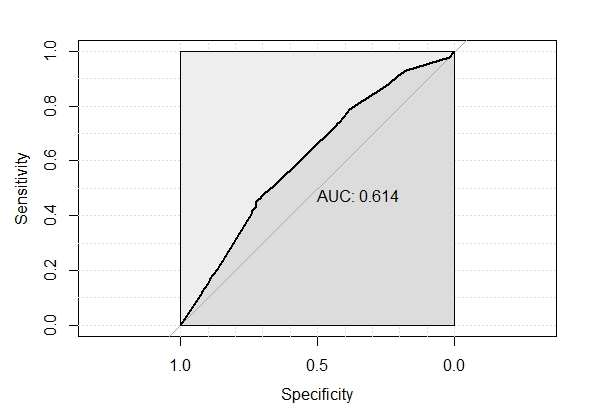
\includegraphics[width=0.55\textwidth]{figs/hiv_roc}
\end{center}
\end{frame}

\begin{frame}{Logistic regression: Prediction summary}
	\begin{itemize}
		\item Just as with linear regression, we get predictions for logistic regression by plugging covariate values into our regression model with estimated coefficients  
		
		\medskip
		
		\item These predictions are naturally on the log-odds scale, but we can transform them to probabilities 
		
		\medskip
		
		\item We can make our predictions binary by choosing a probability cutoff and predicting 0/1 values using that cutoff 
		
		\medskip
		 
		\item We assess the predictive performance of a binary regression model using ROC curves and AUC
	\end{itemize}
\end{frame}
%
%
%



\begin{frame}[c]
	\centering \huge Any Questions?
\end{frame}



\end{document}